\section{动态组合的演算}\label{sec:4}

第3章仅以局部形式建立了空间和时间可组合性。将其推广到整个系统需要将系统分解为组件，每个组件将一个协效应规范与一个见证效应函数配对，使得与共享环境的每一次交互都可归因于其中之一。以下各节为该分解赋予操作语义，并以全局形式建立空间和时间可组合性。

第\S\ref{sec:4.1}节和第\S\ref{sec:4.2}节展示了可以赋予生命周期规则的最小演算，该演算将每个迁移视为原子的、即时的和不会失败的；第\S\ref{sec:4.3}节放弃这三个假设，对迁移可能运行的每个方向分别放弃原子性，允许运行时在迁移开始和结束之间插入的控制流形式，从而得到真实运行时实现的演算；第\S\ref{sec:4.4}节建立该演算的元理论，即保持性、全局时间和空间可组合性、进展性和合流性。

\subsection{组件与纤维}\label{sec:4.1}

本节固定规则所作用的对象：组件；纤维，即携带自身生命周期状态的组件实例化；以及注册表，它保存状态所携带的纤维，并从中读出协效应上下文。

\textbf{组件。}组件以三元组的形式给出，其协效应侧分为从环境中读取的部分和向环境提供的部分。

\begin{definition}\label{def:4.1}
上下文 $\Gamma$ 上同时携带效应和协效应（定义~32）的组件定义如下：
\begin{equation}\label{eq:4.1}
\mathfrak{C}_\Gamma \coloneqq \mathfrak{D}_\Gamma \times \mathfrak{P}_\Gamma \times \mathfrak{E}^*_\Gamma
\end{equation}
表示三元组 $(d, p, e)$，其中：
\begin{itemize}
\item $d: \mathfrak{D}_\Gamma$ 是定义~25 的协效应规范，声明从环境所需的依赖；
\item $p: \mathfrak{P}_\Gamma \coloneqq \mathsf{Set}(K)$ 是供给，声明组件可能提供的协效应键，且 $p$ 之外的键不是其效应函数写入的；
\item $e: \mathfrak{E}^*_\Gamma$ 是定义~8 的见证效应函数，定义组件活跃时贡献的效应以及撤回它们的逆。
\end{itemize}
\end{definition}

这两个声明是同一接口的两个方向，$d$ 是组件从环境读取的部分，$p$ 是组件向环境写入的部分，第\S\ref{sec:4.2}节不允许同一注册表中两个纤维的供给相交。下文始终在 $\Gamma$ 上取下标，协效应上下文是其投影之一（定义~32），因此定义~25 的 $\mathfrak{D}_\Sigma$ 在此写作 $\mathfrak{D}_\Gamma$。

供给的不相交性正是本章与第3.2.3节分道扬镳之处。定义~28 的隔离性允许一个键通过域表解析，因此两个纤维可以在不同域中提供相同的键；携带域的演算会将不相交性放宽为域内的不相交性，并将声明的键对照声明它的纤维的域进行解析。我们在此不引入域，而是在一个共享域中读取每个键，这使得上述不相交性成为正确的条件，且每个键的提供者是唯一的（定义~\ref{def:4.3}）。它所限制的是组件可以被实例化的次数：具有非空供给的组件一次只有一个纤维，因此下面的多次实例化都是针对不提供任何内容的组件，这是只消费或注册其他组件的常见情况。

一个在运行系统中实例化的组件随时间被激活和去激活，因此它携带一个生命周期状态，而迁移将其从一个生命周期状态转移到另一个：激活执行 $e$，在上下文上累积副作用，去激活应用累积器以恢复上下文。在其最简形式中，生命周期是图~\ref{fig:4.1} 的两状态模型，第\S\ref{sec:4.2}节为其给出规则；第\S\ref{sec:4.3}节在每个控制流特性被纳入时对其进行细化。

\begin{figure}[htbp]
\centering
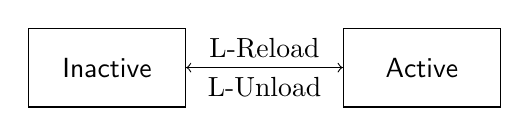
\begin{tikzpicture}[node distance=4cm, auto,
  state/.style={rectangle, draw, minimum width=2cm, minimum height=1cm}]
  \node[state] (inactive) {$\mathsf{Inactive}$};
  \node[state, right of=inactive] (active) {$\mathsf{Active}$};
  \draw[->] (inactive) -- node[above] {L-Reload} (active);
  \draw[->] (active) -- node[below] {L-Unload} (inactive);
\end{tikzpicture}
\caption{基础组件生命周期}\label{fig:4.1}
\end{figure}

\textbf{纤维。}一个组件可以被实例化多次，每次实例化携带自身的生命周期状态。我们将这样的实例化称为纤维。一个纤维记录产生它的组件、它在其下被实例化的纤维、它提供的协效应，以及它处于生命周期中的哪个位置。

\begin{definition}\label{def:4.2}
固定纤维名称的集合 $\mathfrak{N}$。实例化组件 $(d, p, e) \in \mathfrak{C}_\Gamma$ 的纤维是一个元组 $\langle d, p, e, \pi, \sigma, \tau, \theta\rangle$，其中
\begin{itemize}
\item $d: \mathfrak{D}_\Gamma$、$p: \mathfrak{P}_\Gamma$ 和 $e: \mathfrak{E}^*_\Gamma$ 是定义~\ref{def:4.1} 的协效应规范、供给和效应函数；
\item $\pi: \mathfrak{N} \cup \{\mathsf{root}\}$ 是父纤维，即此纤维在其下被实例化的纤维，或根标记 $\mathsf{root}$；
\item $\sigma: \Sigma$ 是纤维自身的协效应表（定义~22），在激活前为空，由其效应运行时写入；
\item $\tau: \{\bot, \top\}$ 是退役标志，$\bot$ 在新纤维中，$\top$ 在编排器退役该纤维后；
\item $\theta: \Theta_\Gamma$ 是生命周期状态，在第\S\ref{sec:4.2}节的两状态模型中为
\end{itemize}
\begin{equation}\label{eq:4.2}
\Theta_\Gamma \coloneqq \mathsf{Inactive} \mid \mathsf{Active}(g, \omega)
\end{equation}
其中 $g: \Gamma \to \Gamma$ 是累积器，$\omega: d \to \mathfrak{N}$ 是已提交视图。
\end{definition}

已提交视图 $\omega$ 将纤维声明的每个键发送到迁移提交时提供该键的纤维名称。第\S\ref{sec:4.3}节用进行中的迁移所需的扩展替换 $\Theta_\Gamma$；定义~\ref{def:4.2} 的其余部分对两者只给出一次，只是 $e$ 在第\S\ref{sec:4.3}节每一层引入的更丰富的效应类型上读取。

\textbf{注册表。}状态将其纤维保存在其名称下，纤维的身份和第3.2节的协效应上下文都是从该安排中读取的。

\begin{definition}\label{def:4.3}
用 $\mathfrak{F}_\Gamma$ 表示 $\Gamma$ 上的纤维集合。状态 $\gamma \in \Gamma$ 携带一个注册表
\begin{equation}\label{eq:4.3}
F_\gamma: \mathfrak{N} \rightharpoonup \mathfrak{F}_\Gamma
\end{equation}
一个有限部分函数，其父指针形成一棵以 $\mathsf{root}$ 为根的树，连同 $\Gamma$ 中没有被任何纤维的 $\sigma$ 命名的其余部分。我们将 $F_\gamma(n)$ 写作 $\gamma(n)$，并在状态明确时用 $n$ 作为下标缩写 $\gamma(n)$ 的字段，因此 $d_n$、$p_n$、$e_n$、$\pi_n$、$\sigma_n$、$\tau_n$、$\theta_n$ 是定义~\ref{def:4.2} 的字段，$g_n$、$\omega_n$ 是 $\theta_n$ 携带的累积器和已提交视图；$\gamma[\theta_n \mapsto \theta']$、$\gamma[n \mapsto \langle \cdots\rangle]$ 和 $\gamma \setminus n$ 分别是在一个字段、一个纤维和一个纤维的存在上与 $\gamma$ 不同的状态。
\end{definition}

纤维的名称赋予它一个经受自身变化的身份：下面的每条规则重写一个纤维的生命周期状态而保持其余不变，因此规则必须指明是哪一个，而有两个字段引用纤维而非描述它们，即父纤维 $\pi$ 和已提交视图 $\omega$。名称是原子：没有规则计算名称、检查其结构或通过除相等之外的任何关系关联两个名称，引入纤维只是抽取一个尚未使用的名称。这就是动态创建的局部名称的学科\cite{ref39}，在此用于纤维身份。

每个纤维拥有一张表意味着协效应上下文是推导出来的而非存储的：它是活跃纤维共同提供的。
\begin{equation}\label{eq:4.4}
\sigma_\gamma \coloneqq \bigcup \{\sigma_m \mid m \in \mathrm{dom}(F_\gamma),\, \theta_m = \mathsf{Active}(-, -)\}
\end{equation}
该并集是良定义的，因为纤维只写入其声明的键，$\mathrm{dom}(\sigma_n) \subseteq p_n$，且不同纤维的供给是不相交的（定义~\ref{def:4.1}），因此每个 $k \in \mathrm{dom}(\sigma_\gamma)$ 恰好位于一个 $\mathsf{Active}$ 纤维的表中，我们将其名称写作 $\mathrm{provider}_k(\gamma) \in \mathfrak{N}$，称为 $k$ 的提供者。因此每个键有一个可能的提供者，由供给而非状态固定。没有规则直接写入 $\sigma_n$：纤维的供给是其自身效应函数执行的集合操作，这些操作落入 $\sigma_n$ 并因此已是 $e_n$ 返回的状态的一部分，它们随累积器再次离开。只有效应的协效应部分以这种方式记录，因为只有协效应部分是其他纤维声明所针对的；在 $\gamma$ 其他地方改变状态的效应由 $g$ 像其他效应一样跟踪，但没有纤维可以在规范中命名它们，因此它们不贡献排序约束。

第3.2.2节的满足关系于是不变地适用，$\gamma \models d$ 缩写 $\sigma_\gamma \models d$。一个键恰好在某个 $\mathsf{Active}$ 纤维安装了它时位于 $\mathrm{dom}(\sigma_\gamma)$ 中，其供给是它可能安装的键而非已经安装的键，因此 $\gamma \models d$ 已要求每个声明的键都有一个 $\mathsf{Active}$ 提供者。仅对 $\mathsf{Active}$ 纤维取并集使得纤维可以在撤回任何内容之前停止提供，第\S\ref{sec:4.3.1}节将其转化为排序规则。

\subsection{基础演算}\label{sec:4.2}

本节给出图~\ref{fig:4.1} 的两状态生命周期的演算，别无其他：每个纤维被比较的目标，以及移动它的五条规则。

\textbf{目标视图。}规则将每个纤维与一个目标进行比较，即它是否应该正在运行以及针对其依赖的哪种解析。目标不仅是纤维本身的属性，因为纤维声明的键是对照整个状态解析的，所以它是该状态上的一个谓词。

\begin{definition}\label{def:4.4}
$n$ 在 $\gamma$ 处的目标视图将每个声明的键映射到其提供者，因此它是全映射 $d_n \to \mathfrak{N}$，当 $n$ 根本不应运行时为 $\bot$：
\begin{equation}\label{eq:4.5}
\mathrm{target}_n(\gamma) \coloneqq \begin{cases}
\bot & \text{if } \tau_n \lor \lnot(\gamma \models d_n) \\
(k \in d_n) \mapsto \mathrm{provider}_k(\gamma) & \text{otherwise}
\end{cases}
\end{equation}
\end{definition}

当每个纤维都已达到其目标视图时，状态是静止的：
\begin{equation}\label{eq:4.6}
\mathrm{quiet}(\gamma) \coloneqq \forall n \in \mathrm{dom}(F_\gamma).\, \begin{cases}
\mathrm{target}_n(\gamma) = \bot & \text{if } \theta_n = \mathsf{Inactive} \\
\mathrm{target}_n(\gamma) = \omega_n & \text{if } \theta_n = \mathsf{Active}(-, \omega_n)
\end{cases}
\end{equation}

目标只回应两件事：退役，通过 $\tau_n$；以及协效应解析，通过 $\gamma \models d_n$ 和 $\mathrm{provider}_k$，每个声明的键从定义~\ref{def:4.1} 的一个共享域中的 $\sigma_\gamma$ 读取。

定义~\ref{def:4.2} 的已提交视图与目标视图具有相同的类型，生命周期的驱动就是比较它们：$\omega_n$ 是 $n$ 激活时对照的解析，$\mathrm{target}_n(\gamma)$ 是它应该运行时对照的解析，下面的每条规则在它们相等或不同时触发。记录提供者而非值使得比较可用，因为否则提供相等值的不同纤维会比较相等。组件读取的值通过视图到达，因为提供者的表持有该值，实现在 \texttt{fiber.committed} 中持有该映射，在 \texttt{fiber.target} 中持有其哈希（第5.1.3节）。

\textbf{规则。}基础演算将每个迁移视为原子的、即时的和不会失败的：激活一步应用其效应函数，去激活一步应用累积器，两者都成功完成。第\S\ref{sec:4.3}节放弃这三个假设。

五条规则生成两个关系。编排规则，前缀 O-，写作 $\gamma \Rightarrow \delta$，是编排器可以执行的动作；其前提说明动作何时合法，而非何时发生。生命周期规则，前缀 L-，写作 $\gamma \longrightarrow \delta$，是系统在前提成立时无需提示即采取的步骤。步骤序列将两者交错，$\longrightarrow^*$ 在下文中仅指生命周期步骤。

\[
\frac{
\begin{array}{c}
n \notin \mathrm{dom}(F_\gamma) \\
\pi \in \mathrm{dom}(F_\gamma) \cup \{\mathsf{root}\} \\
(d, p, e) \in \mathfrak{C}_\Gamma \\
\forall m \in \mathrm{dom}(F_\gamma).\, p \cap p_m = \emptyset
\end{array}
}{
\gamma \Rightarrow \gamma[n \mapsto \langle d, p, e, \pi, \emptyset, \bot, \mathsf{Inactive}\rangle]
}\;\text{O-Insert}
\]

\[
\frac{n \in \mathrm{dom}(F_\gamma)}{
\gamma \Rightarrow \gamma[\tau_n \mapsto \top]
}\;\text{O-Retire}
\]

\[
\frac{
\begin{array}{c}
\tau_n = \top \\
\theta_n = \mathsf{Inactive} \\
\forall m.\, \pi_m \neq n
\end{array}
}{
\gamma \Rightarrow \gamma \setminus n
}\;\text{O-Remove}
\]

插入和退役是仅有的外部输入：编排器请求纤维存在或停止存在，从不直接设置其生命周期状态。O-Retire 对纤维的状态没有条件，因为退役是一个请求，生命周期规则负责执行它。退役与移除分离的原因相同：仍然 $\mathsf{Active}$ 的已退役纤维必须先被去激活，过早移除它会丢弃累积器并造成泄漏。前提 $\forall m.\, \pi_m \neq n$ 通过在父纤维之前移除子纤维来保持树的良构性。O-Insert 的最后一个前提是单源学科的施加之处：一个键有一个可能的提供者，因为编排器不允许第二个声明它的组件进入。

\[
\frac{
\begin{array}{c}
\theta_n = \mathsf{Inactive} \\
\omega = \mathrm{target}_n(\gamma) \neq \bot \\
e_n(\gamma) = (\delta, g)
\end{array}
}{
\gamma \longrightarrow \delta[\theta_n \mapsto \mathsf{Active}(g, \omega)]
}\;\text{L-Reload}
\]

\[
\frac{
\begin{array}{c}
\theta_n = \mathsf{Active}(g, \omega) \\
\mathrm{target}_n(\gamma) \neq \omega \\
g(\gamma) = \delta
\end{array}
}{
\gamma \longrightarrow \delta[\theta_n \mapsto \mathsf{Inactive}]
}\;\text{L-Unload}
\]

L-Reload 与逆一起安装已提交视图；L-Unload 应用逆并丢弃已提交视图。两者由相同的比较驱动：L-Reload 在纤维不持有已提交视图且其目标视图不为 $\bot$ 时触发，L-Unload 在其持有的已提交视图不是其目标视图时触发。这就是第3.2节的响应式规则，从一个同时回应退役和协效应的目标中读出：每当目标视图改变时就发起迁移，无论改变的来源是什么。

\textbf{实例化。}组件在安装其效应时可以实例化另一个组件，这就是插件宿主在插件加载自己的插件时所做的事情。到目前为止的规则将注册表留给编排规则独自处理，因此这样的实例化无处发生。一个原语为其提供场所。

\begin{definition}\label{def:4.5}
$e_n$ 的一次应用，或第\S\ref{sec:4.3.2}节适用时其一次迭代，可以注册一个组件 $(d, p, e) \in \mathfrak{C}_\Gamma$。代替状态映射，它以 $\pi = n$ 对该组件执行 O-Insert，并以其逆作为它产出的 O-Retire。规则抽取名称，受 O-Insert 的新鲜前提约束，并将其交给效应函数。
\end{definition}

逆是退役而非移除，原因是逆必须在到达的任何地方应用。O-Remove 带有前提，因此基于它构建的逆可能无法应用：子纤维仍然 $\mathsf{Active}$ 的父纤维无法运行其累积器，且没有规则会移动子纤维，因为定义~\ref{def:4.4} 不读取纤维树。O-Retire 以 $n \in \mathrm{dom}(F_\gamma)$ 作为其唯一前提。它在注册时的状态处留下的条目是退役的 $\mathsf{Inactive}(\bot)$，持有一个空表，这是引理~\ref{lem:4.4} 的残留条目：它仅在控制字段上与纤维的缺失不同，没有规则区分两者。

退役子纤维设置 $\tau$ 从而将其目标视图变为 $\bot$，此后普通规则将其带回 $\mathsf{Inactive}$。父纤维不需要等待，O-Retire 是无条件的，因此 L-Unload 无论子纤维是否已离开都适用于父纤维。孙纤维逐层到达，子纤维自身的累积器退役子纤维所注册的内容。定理~\ref{thm:4.5} 覆盖了这一级联以及第\S\ref{sec:4.3.1}节沿协效应施加的级联。

\textbf{约束。}有了这一个例外，效应函数所受的约束可以给出。它限定一次应用写入的内容，使得应用它的规则能说明其他所有变化；以及一次应用读取的内容，使得纤维看到它声明的协效应而不更多看到注册表。限定写入正是第\S\ref{sec:4.4}节能将表~\ref{tab:4.1} 读作写入的完整清单的原因。

\begin{definition}\label{def:4.6}
映射 $f: \Gamma \to \Gamma$ 被约束于 $n$，当对于每个 $n \in \mathrm{dom}(F_\gamma)$ 的 $\gamma \in \Gamma$，记 $\delta = f(\gamma)$，
\begin{enumerate}
\item （写入。）$\mathrm{dom}(F_\delta) = \mathrm{dom}(F_\gamma)$，对每个 $m \in \mathrm{dom}(F_\gamma)$ 且 $m \neq n$ 有 $\delta(m) = \gamma(m)$，且 $\delta(n)$ 和 $\gamma(n)$ 仅在 $\sigma$ 上不同；
\item （读取。）两个在 $\sigma_n$、对每个 $m \in \mathrm{dom}(F_\gamma)$ 的限制 $\sigma_m|_{d_n}$、以及没有被任何纤维的表命名的状态部分上相同的状态，被 $f$ 映射到在相同三者上相同的两个状态。
\end{enumerate}
效应函数 $e$ 被约束于 $n$，当其每次应用以及第\S\ref{sec:4.3.2}节适用时的每次迭代，要么注册一个组件（定义~\ref{def:4.5}），要么其状态映射 $\mathrm{pr}_1 \circ e$ 和它产出的逆都被约束于 $n$。每个纤维的效应函数都要求被约束于该纤维。
\end{definition}

注册写入 O-Insert 写入的条目，在其抽取的名称处，不写入其他内容；它作为逆产出的 O-Retire 写入该名称的 $\tau$，不写入其他内容。因此两种应用都不写入已存在纤维的控制字段，除了那一个 $\tau$，也不读取任何控制字段。

条款 (2) 是组件可以读取其声明的值的原因：这些值位于其提供者的表中，因此不读取 $\sigma_n$ 以外的表的效应函数将无法使用其自身的协效应。它不能读取的是 $d_n$ 之外的表，或任何控制字段，这正是阻止组件根据其未声明的纤维的生命周期状态进行分支的原因。

规则是非确定性的：多个纤维可能持有与其目标视图不同的已提交视图，关系不承诺它们之间的顺序。规则也仅是响应式的，没有规则提及调度器；步骤是规则应用的任何序列，因此在所有此类序列上证明的定理对运行时可能采用的任何调度策略都成立。

\subsection{进行中的迁移}\label{sec:4.3}

本节在四个方面扩展基础演算。第一个提供第3.2节要求而第\S\ref{sec:4.2}节无法表达的内容，即一个扩展在其依赖者可能占据的时间间隔上的去激活；其他三个放弃迁移是原子的、即时的和不会失败的理想化假设，而真实运行时中的迁移三者皆非。被放弃的是整个迁移是一个步骤，而不是一个步骤是一次规则应用，四者共享一个结构性后果，在此一次给出：不是一步的迁移需要一个在进行时占据的状态，为其可能运行的每个方向各一个。

\begin{definition}\label{def:4.7}
本节的生命周期状态将 $\Theta_\Gamma$ 替换为
\begin{equation}\label{eq:4.7}
\Theta_\Gamma \coloneqq \mathsf{Inactive}(\zeta) \mid \mathsf{Reloading}(i, g, \omega) \mid \mathsf{Active}(g, \omega) \mid \mathsf{Unloading}(g, \omega, \zeta)
\end{equation}
其中 $i: \mathfrak{E}^{\mathrm{iter}^*}_\Gamma$ 是剩余效应迭代器（下文定义~\ref{def:4.9}），$g: \Gamma \to \Gamma$ 是目前已构建的累积器，$\omega: d \to \mathfrak{N}$ 是已提交视图，$\zeta: \{\bot\} \cup \Xi$ 是结果，由 $\mathsf{Unloading}$ 携带为其去激活所趋向的结果，由 $\mathsf{Inactive}$ 携带为其已达到的结果，要么是 $\bot$，要么是从第\S\ref{sec:4.3.4}节提供的错误集合 $\Xi$ 中抽取的错误。
\end{definition}

纤维在处于携带累积器和已提交视图的三个状态之一时是已安装的，在携带错误结果时是失败的：
\begin{equation}\label{eq:4.8}
\mathrm{installed}_n(\gamma) \coloneqq \theta_n \neq \mathsf{Inactive}(-),\quad \mathrm{failed}_n(\gamma) \coloneqq \exists \xi \in \Xi.\, \theta_n = \mathsf{Inactive}(\xi)
\end{equation}
已安装的纤维 $n$ 在 $\omega_n(k) = m$ 时将 $k$ 解析到 $m$。定义~\ref{def:4.4} 的静止性在更宽的状态空间上读作
\begin{equation}\label{eq:4.9}
\mathrm{quiet}(\gamma) \coloneqq \forall n \in \mathrm{dom}(F_\gamma).\, \begin{cases}
\zeta \neq \bot \lor \mathrm{target}_n(\gamma) = \bot & \text{if } \theta_n = \mathsf{Inactive}(\zeta) \\
\mathrm{target}_n(\gamma) = \omega_n & \text{if } \theta_n = \mathsf{Active}(-, \omega_n) \\
\bot & \text{otherwise}
\end{cases}
\end{equation}

第\S\ref{sec:4.1}节的定义延续到该状态空间，有两处读取需要确定。第一，第\S\ref{sec:4.2}节的 $\mathsf{Inactive}$ 在 O-Insert 的结论中读作 $\mathsf{Inactive}(\bot)$，在 O-Remove 的前提中读作 $\mathsf{Inactive}(-)$。第二，$\sigma_\gamma$ 仍然仅对 $\mathsf{Active}$ 纤维的表取并集，因此一个其迁移在任一方向进行中的纤维通过其持有的 $\omega$ 读取协效应而不提供自己的协效应；其迁移已经写入的键因此还不是依赖者可以激活所对照的键。在两状态演算中这一区分是空的，每个已安装的纤维在那里都是 $\mathsf{Active}$ 的。

图~\ref{fig:4.2} 绘制了这些状态形成的生命周期，以下四个子节提供其边上的规则。

\begin{figure}[htbp]
\centering
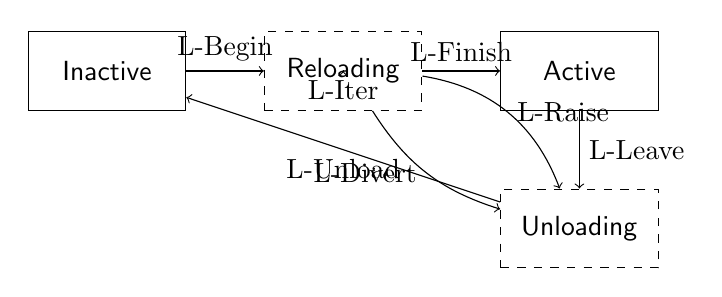
\begin{tikzpicture}[node distance=3cm, auto,
  state/.style={rectangle, draw, minimum width=2cm, minimum height=1cm},
  transstate/.style={rectangle, draw, dashed, minimum width=2cm, minimum height=1cm}]
  \node[state] (inactive) {$\mathsf{Inactive}$};
  \node[transstate, right of=inactive, node distance=3cm] (reloading) {$\mathsf{Reloading}$};
  \node[state, right of=reloading, node distance=3cm] (active) {$\mathsf{Active}$};
  \node[transstate, below of=active, node distance=2cm] (unloading) {$\mathsf{Unloading}$};
  \draw[->] (inactive) -- node[above] {L-Begin} (reloading);
  \draw[->] (reloading) -- node[above] {L-Finish} (active);
  \draw[->] (active) -- node[right] {L-Leave} (unloading);
  \draw[->] (unloading) -- node[below] {L-Unload} (inactive);
  \draw[->, bend left=20] (reloading) to node[below] {L-Iter} (reloading);
  \draw[->, bend right=20] (reloading) to node[left] {L-Divert} (unloading);
  \draw[->, bend left=30] (reloading) to node[right] {L-Raise} (unloading);
\end{tikzpicture}
\caption{带进行中迁移的生命周期；两个迁移状态以虚线框标出}\label{fig:4.2}
\end{figure}

\subsubsection{撤回}\label{sec:4.3.1}

第3.2节要求依赖者在其依赖之后激活，依赖仅在其依赖者去激活之后撤回其供给。前半部分在基础演算中已经成立：激活要求 $\gamma \models d_n$，因此声明 $k$ 的纤维不能在某个纤维活跃提供 $k$ 之前激活。后半部分是实质性的，它必须交付的不仅是状态变化的排序。一个因其提供者即将离开而被拆卸的组件正在运行其自身的拆卸代码，这可能恰好需要正在被撤回的协效应；关闭连接池通常意味着将连接交还给提供它们的一方。后半部分必须交付的是消费者在整个去激活过程中仍然可以读取 $k$，且提供者对 $k$ 的撤回仅在此之后生效。基础演算完全无法交付这一点：其 L-Unload 将供给的移除和逆的运行放在一起，两者之间没有间隔供消费者的拆卸占据。

本层将该步骤一分为二，并用以下条件守护后半部分。

\begin{definition}\label{def:4.8}
纤维 $n$ 在 $\gamma$ 处被依赖，当某个其他已安装的纤维将一个键解析到它：
\begin{equation}\label{eq:4.10}
\mathrm{relied}_n(\gamma) \coloneqq \exists m \in \mathrm{dom}(F_\gamma), k \in d_m.\, m \neq n \land \mathrm{installed}_m(\gamma) \land \omega_m(k) = n
\end{equation}
\end{definition}

\[
\frac{
\begin{array}{c}
\theta_n = \mathsf{Active}(g, \omega) \\
\mathrm{target}_n(\gamma) \neq \omega
\end{array}
}{
\gamma \longrightarrow \gamma[\theta_n \mapsto \mathsf{Unloading}(g, \omega, \bot)]
}\;\text{L-Leave}
\]

\[
\frac{
\begin{array}{c}
\theta_n = \mathsf{Unloading}(g, \omega, \zeta) \\
\lnot\, \mathrm{relied}_n(\gamma) \\
g(\gamma) = \delta
\end{array}
}{
\gamma \longrightarrow \delta[\theta_n \mapsto \mathsf{Inactive}(\zeta)]
}\;\text{L-Unload}
\]

L-Leave 记录去激活的决定而不执行，这使纤维停止提供其协效应，同时保持其自身的已提交视图和其他所有人的已提交视图完好。L-Unload 应用累积器，丢弃已提交视图，使纤维以其携带的结果变为 $\mathsf{Inactive}$；结果为 $\bot$ 直到第\S\ref{sec:4.3.4}节提供其他情况。它是演算中唯一应用累积器的规则。

排序的两半由此由形式的不同部分承载：可见性半由已提交视图承载，L-Unload 以其最后操作丢弃它；排序半由前提 $\lnot\, \mathrm{relied}_n(\gamma)$ 承载，我们称之为守卫，它将 $k$ 的撤回推迟到每个将其解析到 $n$ 的消费者都已离开之后。定理~\ref{thm:4.3} 建立了这两点。

守卫是按绑定施加而非按纤维施加的：$\mathrm{relied}_n(\gamma)$ 测试是否有某个已提交视图命名 $n$，因此不声明 $n$ 的任何键的纤维不是障碍，在另一个域中解析了 $n$ 的某个键的纤维也不是障碍（第3.2.3节）。在第\S\ref{sec:4.2}节的单源学科下，按绑定的读取与更粗的测试 $\exists m \neq n, k \in d_m.\, \mathrm{installed}_m(\gamma) \land k \in p_n$ 一致，一个键在那里只有一个可能的提供者。

这种守卫通常会死锁。使其不死锁的是 $\mathsf{Unloading}$ 连同 $\sigma_\gamma$ 仅对 $\mathsf{Active}$ 纤维取并集：一旦 L-Leave 标记了 $n$，其表离开 $\sigma_\gamma$，因此没有目标视图能再命名 $n$，每个承诺于 $n$ 的消费者自身也在退出的路上。定理~\ref{thm:4.5} 将此转化为守卫总是释放的断言。

守卫沿协效应排序去激活而非沿纤维树：父纤维可以在其子纤维仍然 $\mathsf{Unloading}$ 时运行其逆，因为 $\mathrm{relied}$ 仅涉及已提交视图。父纤维和子纤维因此比定理~\ref{thm:4.3} 排序提供者及其消费者的方式更弱，父纤维和子纤维在环境状态中的效应交集由定义~\ref{def:4.10} 的独立性假设管理。

\subsubsection{迭代}\label{sec:4.3.2}

一次激活可以顺序执行多个效应，去激活必须恢复它们。我们用效应迭代器对此类激活建模，其每次迭代产出修改后的上下文、一个逆和一个续延：

\begin{definition}\label{def:4.9}
定义效应迭代器 $\mathfrak{E}^{\mathrm{iter}}_\Gamma$ 和见证效应迭代器 $\mathfrak{E}^{\mathrm{iter}^*}_\Gamma$ 为以下递归类型：
\begin{equation}\label{eq:4.11}
\mathfrak{E}^{\mathrm{iter}}_\Gamma \coloneqq \mu \mathfrak{I}.\, \Gamma \to \Gamma \times (\Gamma \to \Gamma) \times \mathsf{Maybe}(\mathfrak{I})
\end{equation}
\begin{equation}\label{eq:4.12}
\mathfrak{E}^{\mathrm{iter}^*}_\Gamma \coloneqq \mu \mathfrak{I}.\, (e: \Gamma \to \Gamma \times (\Gamma \to \Gamma) \times \mathsf{Maybe}(\mathfrak{I})) \times ((\gamma: \Gamma) \to (\mathbf{let}\,(\delta, g, o) = e(\gamma)\,\mathbf{in}\, g(\delta) \simeq \gamma))
\end{equation}
其中 $e(\gamma)$ 产出三元组 $(\delta, g, o)$，表示：
\begin{itemize}
\item $\delta$ 是新上下文；
\item $g$ 是当前效应的逆函数；
\item $o$ 指示续延：
\begin{itemize}
\item $\mathsf{Nothing}$ 表示迭代终止；
\item $\mathsf{Just}(i)$ 提供下一次迭代。
\end{itemize}
\end{itemize}
见证在定义~33 的 $\simeq$ 处读取，正如定义~37 读取 $\mathfrak{E}^*_\Gamma$ 的见证：$i \in \mathfrak{E}^{\mathrm{iter}}_\Gamma$ 在 $i$ 尊重 $\simeq$ 且其产出的每个 $g$ 尊重 $\simeq$ 并满足上述条款时属于 $\mathfrak{E}^{\mathrm{iter}^*}_\Gamma$。三元组逐分量比较，$\mathsf{Nothing}$ 仅与 $\mathsf{Nothing}$ 比较，$\mathsf{Just}(i)$ 在 $i \simeq i'$ 时与 $\mathsf{Just}(i')$ 比较，$\simeq$ 在迭代器上是满足这些条款的最大关系。将 $\simeq$ 取为 $\Gamma$ 上的相等性即可精确恢复读取。
\end{definition}

效应迭代器变换 $\mathrm{effect}^{\mathrm{iter}}_\Gamma$ 通过递归调用将 $\mathrm{effect}_\Gamma$ 扩展到迭代器结构：

\begin{definition}\label{def:4.10}
定义效应迭代器变换 $\mathrm{effect}^{\mathrm{iter}}_\Gamma$ 为：
\begin{equation}\label{eq:4.13}
\mathrm{effect}^{\mathrm{iter}}_\Gamma: \mathfrak{E}^{\mathrm{iter}}_\Gamma \to \partial\Gamma \to \partial^2\Gamma
\end{equation}
\[
\mathrm{effect}^{\mathrm{iter}}_\Gamma = i \mapsto (\gamma, \varphi) \mapsto \mathbf{let}\,(\delta, g, o) = i(\gamma)\,\mathbf{in}\, \mathbf{let}\,t = \mathrm{track}_\Gamma(g, \mathrm{pr}_1 \circ i)\,\mathbf{in}\, \mathbf{match}\,o
\]
\[
\mid \mathsf{Nothing} \Rightarrow ((\delta, \varphi \circ g), t)
\]
\[
\mid \mathsf{Just}(i') \Rightarrow \mathbf{let}\,(s, r) = \mathrm{effect}^{\mathrm{iter}}_\Gamma(i')(\delta, \varphi \circ g)\,\mathbf{in}\, (s, t \circ r)
\]
\end{definition}

在每次迭代中，逆 $g$ 按应用顺序组合到 $\varphi$ 上，因此累积器 $\varphi \circ g_1 \circ \cdots \circ g_k$ 在应用时自然以后进先出的顺序恢复效应。因为 $\mathrm{effect}^{\mathrm{iter}}_\Gamma$ 落在与 $\mathrm{effect}_\Gamma$ 相同的 $\partial\Gamma \to \partial^2\Gamma$ 中，迭代器本身就是一种效应，可以在效应可用的任何地方使用。组件的整个激活就是这样一种使用，这就是本节其余部分形式化的内容，实现在每个变异点都接受迭代器（第5.1.1节）。$\mathsf{Maybe}(\mathfrak{E}^{\mathrm{iter}})$ 续延在任意两次连续迭代之间提供了一个边界，在边界处上下文是到目前为止的迭代所产生的，累积器恢复这些而不更多。在这个意义上，效应迭代器是一个具体化的定界续延，主流语言通过 \texttt{yield} 运算符暴露的结构\cite{ref43}，因此模型直接映射到它们已提供的生成器。

在演算中，定义~\ref{def:4.2} 的 $e_n$ 从此处在 $\mathfrak{E}^{\mathrm{iter}^*}_\Gamma$ 上读取，用迭代器替代原子效应函数将基础 L-Reload 分裂为轨迹经过的一个开始状态，并给纤维从该状态退出的第二种方式。

\[
\frac{
\begin{array}{c}
\theta_n = \mathsf{Inactive}(\bot) \\
\omega = \mathrm{target}_n(\gamma) \neq \bot
\end{array}
}{
\gamma \longrightarrow \gamma[\theta_n \mapsto \mathsf{Reloading}(e_n, \mathrm{id}_\Gamma, \omega)]
}\;\text{L-Begin}
\]

\[
\frac{
\begin{array}{c}
\theta_n = \mathsf{Reloading}(i, g, \omega) \\
\mathrm{target}_n(\gamma) \neq \omega \\
(\delta, h) = (\gamma, \mathrm{id}_\Gamma) \lor i(\gamma) = (\delta, h, -)
\end{array}
}{
\gamma \longrightarrow \delta[\theta_n \mapsto \mathsf{Unloading}(g \circ h, \omega, \bot)]
}\;\text{L-Divert}
\]

\[
\frac{
\begin{array}{c}
\theta_n = \mathsf{Reloading}(i, g, \omega) \\
\mathrm{target}_n(\gamma) = \omega \\
i(\gamma) = (\delta, h, \mathsf{Just}(i'))
\end{array}
}{
\gamma \longrightarrow \delta[\theta_n \mapsto \mathsf{Reloading}(i', g \circ h, \omega)]
}\;\text{L-Iter}
\]

\[
\frac{
\begin{array}{c}
\theta_n = \mathsf{Reloading}(i, g, \omega) \\
\mathrm{target}_n(\gamma) = \omega \\
i(\gamma) = (\delta, h, \mathsf{Nothing})
\end{array}
}{
\gamma \longrightarrow \delta[\theta_n \mapsto \mathsf{Active}(g \circ h, \omega)]
}\;\text{L-Finish}
\]

每次迭代将新产出的逆组合到累积器上为 $g \circ h$，遵循定义~\ref{def:4.10}，因此累积器以后进先出的顺序应用逆。在任意两次连续迭代之间，系统可以在目标视图改变时转移迁移，将目前已累积的逆应用于恢复上下文。L-Divert 像每个其他去激活一样路由通过 $\mathsf{Unloading}$，而不是在原位应用累积器，它在那里遇到的守卫是空的，一个从未 $\mathsf{Active}$ 的纤维不提供任何内容也不出现在任何已提交视图中。它的两个选择中的第一个中止纤维持有的迭代，这只有迭代边界才使之可能，因此转移可能落下的粒度就是迭代器的粒度；第二个让该迭代着陆，第\S\ref{sec:4.3.3}节正是需要它的地方。

普通的效应函数（$\mathfrak{E}_\Gamma$）是退化情况，其第一次迭代已产出 $\mathsf{Nothing}$。这样的迁移仍然经过 $\mathsf{Reloading}$，L-Divert 仍然在那里适用，但累积器是 $\mathrm{id}_\Gamma$ 且没有迭代运行过，因此没有恢复任何内容，迁移要么安装其全部效应，要么一个都不安装。

\subsubsection{异步性}\label{sec:4.3.3}

到目前为止的层允许环境在迭代之间移动，并假设每次迭代本身即时完成，其启动和着陆是一个步骤。我们抽象地建模非即时性：一次迭代产出类型为 $\mathsf{Future}(A)$ 的值，其中 $\mathsf{Future}$ 是一个不透明类型构造子，其定义性质是在提交和解析之间外部状态可能改变。

在此模型下，一次迭代在一个状态启动并在另一个状态着陆，而纤维在飞行中处于 $\mathsf{Reloading}$。本层增加的是惯性：一旦启动，迭代就着陆，其着陆不能被拒绝。因此在飞行期间转向的目标视图不能通过中止迭代来回应，只有着陆一个迭代的 L-Divert 的替代选择仍然可用：迭代着陆，纤维随后去激活。因此本层不增加规则，也不增加规则匹配的类型；在 $\Gamma$ 的粒度上惯性就是其全部内容，它采取对 L-Divert 的哪个替代选择宿主可以采取的限制形式。

那个替代选择正是基础演算无法表达的。在那里，目标视图已转向的迁移在发现转向的同一步中被撤销；这里飞行中的迭代必须先着陆，因此纤维需要在运行其逆时有一个地方待，唯一合理的位置是 $\mathsf{Unloading}$ 持有迭代产出的逆。改为路由通过 $\mathsf{Active}$ 会让纤维在一个步骤的长度内提供其协效应，并迫使依赖者激活对照一个已经在离开的组件。这就是实现中重载和卸载的互链。

去激活也可以通过复合而非规则直接链回激活。L-Unload 对目标视图没有前提，因此无论纤维去激活期间目标视图变成什么，累积器运行且纤维变为 $\mathsf{Inactive}$，L-Begin 可以立即从那里开始新的迁移。

\subsubsection{失败}\label{sec:4.3.4}

到目前为止的每条规则都假设其运行的效应成功，而运行时做不到这一点。组件安装的效应到达跟踪它们的上下文之外，到达的部分可能拒绝：一个已绑定的端口、一个不存在的文件、一个不响应的对端。失败的迁移仍然必须使纤维的效应被恢复而非搁浅。

设 $\Xi$ 为错误集合，将定义~\ref{def:4.9} 的效应迭代器细化使得迭代可以抛出异常而非产出三元组：
\begin{equation}\label{eq:4.15}
\mathfrak{E}^{\mathrm{fail}}_\Gamma \coloneqq \mu \mathfrak{I}.\, \Gamma \to \mathsf{Either}(\Xi, \Gamma \times (\Gamma \to \Gamma) \times \mathsf{Maybe}(\mathfrak{I}))
\end{equation}
\begin{equation}\label{eq:4.16}
\mathfrak{E}^{\mathrm{fail}^*}_\Gamma \coloneqq \mu \mathfrak{I}.\, (e: \Gamma \to \mathsf{Either}(\Xi, \Gamma \times (\Gamma \to \Gamma) \times \mathsf{Maybe}(\mathfrak{I}))) \times ((\gamma: \Gamma) \to (\mathbf{let}\,\mathsf{Right}(\delta, g, o) = e(\gamma)\,\mathbf{in}\, g(\delta) \simeq \gamma))
\end{equation}
见证仅约束 $\mathsf{Right}$ 的情况，在模式不匹配处是空的，抛出异常没有需要撤销的内容，$\mathsf{Reloading}$ 携带的 $i$ 从此处在 $\mathfrak{E}^{\mathrm{fail}^*}_\Gamma$ 上读取。定义~\ref{def:4.10} 的提升以抛出异常替代三元组传播的方式延续，因此抛出异常的迭代器可以在效应可用的任何地方使用，正如普通迭代器一样。本层增加一条规则并将定义~\ref{def:4.7} 的第二个结果投入使用，O-Remove 不需要加宽即可接受它。L-Iter、L-Finish 和 L-Divert 的前提在它们匹配的三元组周围读取 $\mathsf{Right}$。抛出异常是迭代所做的事情，因此规则是从 $\mathsf{Reloading}$ 的出口。

\[
\frac{
\begin{array}{c}
\theta_n = \mathsf{Reloading}(i, g, \omega) \\
i(\gamma) = \mathsf{Left}(\xi)
\end{array}
}{
\gamma \longrightarrow \gamma[\theta_n \mapsto \mathsf{Unloading}(g, \omega, \xi)]
}\;\text{L-Raise}
\]

L-Raise 在记录之前先恢复。纤维路由进入 $\mathsf{Unloading}$ 携带错误作为其结果，到失败迭代为止构建的累积器在那里应用，纤维到达 $\mathsf{Inactive}(\xi)$ 时没有安装任何内容，在与中止的 L-Divert 所产生的状态仅在纤维携带的结果上不同的状态处。像每个其他去激活一样路由失败是使得每个结果仅通过 L-Unload 可达的单一事实，定理~\ref{thm:4.1} 正以此为基础。L-Begin 以 $\mathsf{Inactive}(\bot)$ 为前提，因此生命周期不从错误结果重新进入；这是结果的实质，它阻止了一个效应函数已表明在运行时所对照的状态中不可靠的纤维被重试对照不变的环境。失败的纤维也不阻碍任何东西：它是 $\mathsf{Inactive}$ 的，因此不携带已提交视图，也不能使 $\mathrm{relied}$ 成立。

失败记录在纤维上而非传播到其父纤维，因此迁移失败的组件让其兄弟继续运行，这是插件宿主想要的行为，也是结果按纤维设置而非整个状态属性的原因。

\subsection{元理论}\label{sec:4.4}

第\S\ref{sec:4.3}节提供十条规则：第\S\ref{sec:4.2}节的三条编排规则；L-Begin、L-Iter 和 L-Finish 用于激活；L-Divert 和 L-Raise 用于激活可能提前结束的两种方式；以及 L-Leave 和 L-Unload 用于去激活。本节从这些规则中以全局形式读出可组合性的两个维度，一个纤维的保证在其他纤维之间的任何操作下都成立，并添加只有整个系统才能被要求的内容：它总是到达其目标所要求的配置，且该配置是静态组装本会产生的配置。下面的每个性质都是步骤序列的性质，因此我们索引步骤并从该索引读取状态的字段。

两个约定将第3.3.2节延续到本节。下面状态之间的每个相等都在定义~33 的观察等价 $\simeq$ 下读取，正如引理~38 读取第3.1节的那些，效应函数所受的见证条件是定义~37 给出的那个，对迭代器按定义~\ref{def:4.9} 读取，对注册迭代在下文的 $\approx$ 处读取。

\begin{definition}\label{def:4.11}
用 $t$ 索引步骤，使得 $\gamma_t$ 是前 $t$ 步到达的状态，并记
\begin{equation}\label{eq:4.17}
\mathrm{step}_t \coloneqq r(n)
\end{equation}
为在 $\gamma_t$ 处采取的步骤：它应用的规则 $r$，十条之一，以及它应用该规则的名称 $n \in \mathfrak{N}$。序列从一个 $\gamma_0$ 开始，$\mathrm{dom}(F_0) = \emptyset$，因此每个纤维通过 O-Insert 进入存在，无论是编排器的还是迭代所采取的（定义~\ref{def:4.5}）。$\gamma_t$ 的字段携带索引作为上标，因此 $\theta^t_n$、$\omega^t_n$、$\sigma^t_n$、$g^t_n$ 和 $i^t_n$ 是 $n$ 在 $\gamma_t$ 处的生命周期状态、已提交视图、表、累积器和剩余迭代器，$F^t$ 和 $\sigma^t$ 是 $\gamma_t$ 本身的注册表和协效应上下文，即定义~\ref{def:4.3} 在那里读取的 $F_\gamma$ 和 $\sigma_\gamma$。谓词以状态为参数、其余为下标，因此 $\mathrm{installed}^t_n$、$\mathrm{target}^t_n$、$\mathrm{relied}^t_n$ 和 $\mathrm{quiet}^t$ 是定义~\ref{def:4.4}、定义~\ref{def:4.7} 和定义~\ref{def:4.8} 在 $\gamma_t$ 处的谓词。$n$ 的一个片段是索引的最大区间 $[b, u]$，在其中 $\mathrm{installed}^t_n$ 成立。它在 $b$ 处开启，其中 $b > 0$ 且 $\lnot\,\mathrm{installed}^{b-1}_n$，空的 $F_0$ 使得开始时没有纤维被安装；它在 $u$ 处关闭当 $\mathrm{installed}^u_n$ 且 $\lnot\,\mathrm{installed}^{u+1}_n$，最终片段不需要这样做。
\end{definition}

第\S\ref{sec:4.3}节的每条规则结论的形状为 $\gamma \longrightarrow \delta[\cdots]$，其中前提从 $\gamma$ 计算 $\delta$ 并在未计算时将其留作 $\gamma$，方括号编辑注册表的命名字段。两半分别命名，两者都是整个 $\Gamma$ 上的映射。在 $\gamma_t$ 处由作用于 $n$ 的规则所采取的步骤的状态映射为
\begin{equation}\label{eq:4.18}
\Psi_t \coloneqq \begin{cases}
\mathrm{pr}_1 \circ i & \mbox{在 L-Iter、L-Finish 和着陆的 L-Divert 处} \\
g & \mbox{在 L-Unload 处} \\
\mathrm{id}_\Gamma & \mbox{在所有其他规则处}
\end{cases}
\end{equation}
其中 $i$ 和 $g$ 是 $\theta^t_n$ 携带的迭代器和累积器，编辑 $\mathrm{edit}_t: \Gamma \to \Gamma$ 是方括号作为函数读取，赋予它命名的字段以在 $\gamma_t$ 处前提计算的值。两者因此由 $\mathrm{step}_t$ 连同 $\gamma_t$ 固定并在每个状态上定义，这正是定理~\ref{thm:4.7} 和引理~\ref{lem:4.9} 能在远离 $\gamma_t$ 处求值它们的原因。每一步分解为
\begin{equation}\label{eq:4.19}
\gamma_{t+1} = \mathrm{edit}_t(\Psi_t(\gamma_t))
\end{equation}
例如在 L-Unload 处，$\mathrm{edit}_t$ 是 $[\theta_n \mapsto \mathsf{Inactive}(\zeta)]$，在 O-Remove 处是移除 $\setminus n$，这就是为什么后半是编辑而非赋值。字段沿着相同的接缝划分：表 $\sigma_m$，一旦创建 $m$ 的 O-Insert 将其设为空后不再有 $\mathrm{edit}_t$ 写入；控制字段 $\theta_m$、$\tau_m$、$\pi_m$、$d_m$、$p_m$、$e_m$ 连同 $\mathrm{dom}(F_\gamma)$，除了通过定义~\ref{def:4.5} 的原语外不再有 $\Psi_t$ 写入。记 $\gamma \approx \delta$ 当两个状态在除控制字段外的一切上相同。

关系 $\approx$ 不是定义~33 的 $\simeq$，两者互不精化，因为各自忘记了对方必须保留的内容。恢复精确性是关于效应的声明，因此 $\approx$ 精确比较表和环境状态，仅忘记注册表记录哪个纤维安装了它们。规则读取控制字段来决定是否适用，因此 $\simeq$ 必须保留它们，本节将其读取为定义~33 与注册表域上的一致以及每个纤维的每个控制字段上的一致的合取：
\begin{equation}\label{eq:4.20}
\gamma \simeq \delta \coloneqq \sigma_\gamma \simeq \sigma_\delta \land \mathrm{dom}(F_\gamma) = \mathrm{dom}(F_\delta) \land \forall n, c \in \{\theta, \tau, \pi, d, p, e\}.\, c(\gamma(n)) \simeq c(\delta(n))
\end{equation}
函数类型的字段，如 $e_n$ 和 $\theta_n$ 内部的 $g$，按定义~36 比较映射的方式比较，迭代器按定义~\ref{def:4.9} 比较两个迭代器的方式比较，其他类型的字段按相等性比较。下面的结果在两个关系下都成立，一个用于状态的每一半，引理~\ref{lem:4.3} 对所有十条规则一次性建立 $\simeq$ 的那一半。

表~\ref{tab:4.1} 是第\S\ref{sec:4.3}节的十条规则作为此类写入的读取。累积器、已提交视图和剩余迭代器是 $\theta_n$ 的组成部分，因此第三列也记录对它们的写入，$h$ 在那里命名第四列的迭代产出的逆，$\mathrm{id}_\Gamma$ 在 L-Divert 中止该迭代处。在从迭代器构建的 $\Psi_t$ 注册纤维（定义~\ref{def:4.5}）处，该注册在其抽取的名称处携带 O-Insert 行的写入，累积器退役一个纤维的 L-Unload 携带 O-Retire 行的写入。下面的每个分情况分析都是表中的查找，五个查找频繁出现足以命名。

\begin{table}[htbp]
\centering
\caption{规则作为对其所作用的纤维 $n$ 的写入，其中 $\mathrm{step}_t$ 是在 $n$ 处应用该规则}\label{tab:4.1}
\begin{tabular}{lllll}
\hline
规则 & $\theta^t_n$ & $\theta^{t+1}_n$ & $\Psi_t$ & 编辑的控制字段 \\
\hline
O-Insert & undefined & $\mathsf{Inactive}(\bot)$ & $\mathrm{id}_\Gamma$ & $\mathrm{dom}(F_\gamma)$ \\
O-Retire & unconstrained & unchanged & $\mathrm{id}_\Gamma$ & $\tau_n$ \\
O-Remove & $\mathsf{Inactive}(-)$ & undefined & $\mathrm{id}_\Gamma$ & $\mathrm{dom}(F_\gamma)$ \\
L-Begin & $\mathsf{Inactive}(\bot)$ & $\mathsf{Reloading}(e_n, \mathrm{id}_\Gamma, \omega)$ & $\mathrm{id}_\Gamma$ & $\theta_n$ \\
L-Iter & $\mathsf{Reloading}(i, g, \omega)$ & $\mathsf{Reloading}(i', g \circ h, \omega)$ & $\mathrm{pr}_1 \circ i$ & $\theta_n$ \\
L-Finish & $\mathsf{Reloading}(i, g, \omega)$ & $\mathsf{Active}(g \circ h, \omega)$ & $\mathrm{pr}_1 \circ i$ & $\theta_n$ \\
L-Divert & $\mathsf{Reloading}(i, g, \omega)$ & $\mathsf{Unloading}(g \circ h, \omega, \bot)$ & $\mathrm{id}_\Gamma$ 或 $\mathrm{pr}_1 \circ i$ & $\theta_n$ \\
L-Raise & $\mathsf{Reloading}(i, g, \omega)$ & $\mathsf{Unloading}(g, \omega, \xi)$ & $\mathrm{id}_\Gamma$ & $\theta_n$ \\
L-Leave & $\mathsf{Active}(g, \omega)$ & $\mathsf{Unloading}(g, \omega, \bot)$ & $\mathrm{id}_\Gamma$ & $\theta_n$ \\
L-Unload & $\mathsf{Unloading}(g, \omega, \zeta)$ & $\mathsf{Inactive}(\zeta)$ & $g$ & $\theta_n$ \\
\hline
\end{tabular}
\end{table}

\begin{lemma}\label{lem:4.1}
连同定义~\ref{def:4.6} 读取表~\ref{tab:4.1}，对于每一步 $t$ 和 $\gamma_t$ 处的所有纤维 $m$、$n$：
\begin{enumerate}
\item $\sigma^{t+1}_m \neq \sigma^t_m$ 仅在步骤 $t$ 作用于 $m$ 处，写入位于 $\Psi_t$ 内部；
\item $\omega_n$ 仅在 $\mathrm{step}_t = \text{L-Begin}(n)$ 处进入存在，仅在 $\mathrm{step}_t = \text{L-Unload}(n)$ 处消失，因此 $\omega^t_n$ 在 $n$ 的一个片段中对 $t$ 是常量；
\item $\Psi_t = g^t_n$ 仅在 $\mathrm{step}_t = \text{L-Unload}(n)$ 处，没有其他步骤将 $g_n$ 应用于状态；
\item $\lnot\,\mathrm{installed}^t_n \land \mathrm{installed}^{t+1}_n \Rightarrow \mathrm{step}_t = \text{L-Begin}(n)$，且 $\mathrm{installed}^t_n \land \lnot\,\mathrm{installed}^{t+1}_n \Rightarrow \mathrm{step}_t = \text{L-Unload}(n)$；
\item $\pi_n$、$d_n$、$p_n$ 和 $e_n$ 随 $n$ 的条目进入存在且此后不再被写入，$\tau_n$ 是单调的，仅在 $\top$ 处写入且仅由 O-Retire 写入。
\end{enumerate}
\end{lemma}

\begin{proof}
设步骤 $t$ 在 $n$ 处应用 $r$。由定义~\ref{def:4.11}，它分解为 $\mathrm{edit}_t \circ \Psi_t$，其中 $\mathrm{edit}_t$ 写入表~\ref{tab:4.1} 第五列命名的字段而不写入其他，$\Psi_t$ 是 $\mathrm{id}_\Gamma$、$n$ 的一次迭代应用或累积器 $g^t_n$，后者是那些迭代产出的逆的复合。三者由定义~\ref{def:4.6} 都约束于 $n$，因此 $\Psi_t$ 不写入 $\gamma_t$ 处的任何纤维的字段但 $\sigma_n$，连同注册添加的条目和其逆写入的 $\tau$。两半因此划分写入，每个条款是在一个字段处读取该划分。第二列和第三列的一种读取使用了两次：$\mathsf{Inactive}$ 是不携带已提交视图的唯一生命周期状态，L-Begin 是唯一从中引出的规则，L-Unload 是唯一引向它的规则，而其他每行将其前提的 $\omega$ 不变地带入其结论。

(1) $\mathrm{edit}_t$ 不写入表，第五列未命名任何表，$\Psi_t$ 对存在的 $m \neq n$ 不写入 $\sigma_m$。因此 $\sigma_m$ 仅在 $m = n$ 处移动，且仅在 $\Psi_t$ 内部。

(2) $\omega_n$ 是 $\theta_n$ 的组成部分，仅有 $\mathrm{edit}_t$ 写入且仅在步骤作用的纤维处，因此按上述读取，$\omega_n$ 在 $n$ 的 L-Begin 处进入存在，在 $n$ 的 L-Unload 处消失。$n$ 的片段是 $\mathrm{installed}_n$ 成立的区间，因此是 $\omega_n$ 定义于其上的区间，两条规则都不落入其内部。

(3) 第四列，累积器仅在 L-Unload 处出现：其他规则取前向映射 $\mathrm{pr}_1 \circ i$ 或 $\mathrm{id}_\Gamma$，没有 $\mathrm{edit}_t$ 将映射应用于状态。

(4) $\mathrm{installed}_n$ 是 $\theta_n \neq \mathsf{Inactive}(-)$，按上述读取 L-Begin 和 L-Unload 是前提和结论在 $\theta_n$ 是否为 $\mathsf{Inactive}$ 上不同的唯一规则。作用于某个 $m \neq n$ 的步骤不写入 $\theta_n$，注册添加的条目在 $\gamma_t$ 处不存在的名称处。

(5) 第五列没有行命名 $\pi$、$d$、$p$ 或 $e$；它们随 O-Insert 添加的条目进入存在，其结论写入，注册所采取的 O-Insert 也一样。仅 O-Retire 在 $\top$ 处写入 $\tau$，无论是编排器采取的还是注册的逆（定义~\ref{def:4.5}）；O-Insert 在尚未存在的名称处设置 $\tau = \bot$，因此没有步骤将 $\tau$ 返回 $\bot$。
\end{proof}

三个进一步的查找说明规则不能看到什么。第一个是它们仅通过上述观察读取状态，因此整个演算下降到 $\Gamma/{\simeq}$。

\begin{lemma}\label{lem:4.2}
（$\simeq$-不变性。）设 $\gamma \simeq \gamma'$ 如上所读。则第\S\ref{sec:4.3}节的规则在 $\gamma$ 处作用于 $n$ 当且仅当它在 $\gamma'$ 处作用于 $n$，且两个应用到达的状态再次由 $\simeq$ 关联。
\end{lemma}

\begin{proof}
第\S\ref{sec:4.3}节的每个前提属于四种之一，每种读取关系保留的组成部分。将 $\theta_n$ 或 $\tau_n$ 与模式匹配的前提，以及 O-Remove 的前提 $\forall m.\, \pi_m \neq n$ 读取控制字段。O-Insert 的前提 $(d, p, e) \in \mathfrak{C}_\Gamma$ 和 $\forall m.\, p \cap p_m = \emptyset$ 读取 $d$、$p$ 和 $e$。提及 $\mathrm{target}_n$ 或 $\mathrm{relied}_n$ 的前提读取 $\tau_n$、$\theta_m$ 内部的已提交视图，以及 $\mathrm{dom}(\sigma_\gamma)$，定义~\ref{def:4.3} 从 $\theta_m$ 和 $\mathrm{dom}(\sigma_m)$ 计算，定义~33 仅在两个协效应上下文的域一致时关联它们。其余前提读取 $\mathrm{dom}(F_\gamma)$。没有前提在 $\simeq_k$ 下而非 $\sigma_\gamma(k)$ 的值上读取，因此没有前提分离两个 $\simeq$-关联的状态。

对于结论，由定义~\ref{def:4.11}，$\gamma_{t+1} = \mathrm{edit}_t(\Psi_t(\gamma_t))$。$\mathrm{edit}_t$ 赋予的值是其前提匹配的组成部分，在上面的段落和定义~\ref{def:4.9} 的关联下在两个状态处关联，后者关联迭代器在 $\simeq$-关联状态产出的三元组。且 $\Psi_t$ 尊重 $\simeq$：它是 $\mathrm{id}_\Gamma$，或 $e_n$ 的迭代，定义~\ref{def:4.9} 要求其尊重 $\simeq$，或 $\theta_n$ 内部的累积器，由每个尊重 $\simeq$ 的逆按相同定义组合而成。
\end{proof}

状态携带的名称由两个上述观察读取，$\mathrm{dom}(F_\gamma)$ 和控制字段的索引，抽取名称的规则抽取任何尚未使用的名称（定义~\ref{def:4.5}）。因此在 $\simeq$ 下读取下面的结果也要求在重命名下读取它们，这是第\S\ref{sec:4.1}节兑现的学科。

\begin{lemma}\label{lem:4.3}
（等变性。）设 $\chi: \mathfrak{N} \to \mathfrak{N}$ 为双射，设 $\chi \cdot \gamma$ 是携带注册表 $F_\gamma \circ \chi^{-1}$ 的状态，$\pi_m$ 或 $\omega_m$ 中出现的每个名称被其像替换。则 $\chi \cdot \gamma$ 是一个状态，在 $\gamma$ 良构处良构，$\mathrm{step}_t = r(n)$ 将 $\gamma_t$ 带到 $\gamma_{t+1}$ 当且仅当 $r(\chi(n))$ 将 $\chi \cdot \gamma_t$ 带到 $\chi \cdot \gamma_{t+1}$。
\end{lemma}

\begin{proof}
前提仅通过将名称与另一个比较来读取名称，无论是直接的，如 O-Insert 的新鲜性 $n \notin \mathrm{dom}(F_\gamma)$ 和 O-Remove 的 $\forall m.\, \pi_m \neq n$，还是通过名称表，如 $\mathrm{target}_n$ 和 $\mathrm{relied}_n$ 读取 $\pi_m$ 和 $\omega_m$。双射保持每个此类比较。规则写入的唯一名称是 O-Insert 设置的 $\pi$ 和 L-Begin 设置的 $\omega$，两者都取自其前提读取的内容，因此写入与 $\chi$ 交换；效应函数根本不写入名称，仅通过定义~\ref{def:4.5} 的原语抽取，定义~\ref{def:4.6} 将其约束于该原语添加的条目。良构性（定义~\ref{def:4.8}）是四个比较名称与名称的条件。
\end{proof}

序列及其重命名因此以相同顺序采取相同的规则并到达仅 $\chi$ 不同的状态。在注册抽取的名称上一致而其余一致的两个序列据此被识别，下面的结果在识别它们的重命名下读取。

第二个查找是剥夺了除名称之外一切的条目对规则是不可见的，这使得定义~\ref{def:4.5} 可以在恢复的状态没有纤维的地方退役一个纤维，引理~\ref{lem:4.9} 移除已删除片段所做的注册。

\begin{lemma}\label{lem:4.4}
（残留条目。）称 $n$ 在 $\gamma$ 处是残留的，当 $\tau_n = \top$、$\theta_n = \mathsf{Inactive}(\bot)$、$\sigma_n = \emptyset$ 且没有 $m$ 满足 $\pi_m = n$；残留条目满足 $\gamma \approx \gamma \setminus n$。如果 $n$ 在 $\gamma$ 处是残留的，则对每条规则和每个 $m \neq n$：
\begin{enumerate}
\item 在 $\gamma$ 处作用于 $m$ 的规则在 $\gamma \setminus n$ 处作用于 $m$，两者到达的状态仅在 $n$ 处的条目不同，该条目保持残留；
\item 反之，在 $\gamma \setminus n$ 处作用于 $m$ 的规则在 $\gamma$ 处适用，除非它是抽取名称 $n$ 或声称 $p_n$ 的键的 O-Insert。
\end{enumerate}
\end{lemma}

\begin{proof}
残留的 $n$ 不贡献于任何作用于 $m \neq n$ 的规则的前提读取的观察。它不是 $\mathsf{Active}$ 的，因此 $\sigma_n$ 不进入 $\sigma_\gamma$，$n$ 不是任何键的提供者，$\gamma \models d_m$ 和 $\mathrm{target}_m$ 不受影响；$\mathrm{installed}_n$ 失败，因此 $n$ 不贡献 $\mathrm{relied}_m$ 的析取项；没有 $\pi_{m'}$ 命名 $n$，因此 $m$ 的 O-Remove 的前提 $\forall m'.\, \pi_{m'} \neq m$ 不受影响；$\theta_n$、$\tau_n$ 和 $\pi_n$ 仅被作用于 $n$ 的规则读取。条款 (2) 除外的前提是移除放宽的两个前提，不存在的名称是新鲜的，不存在的供给与每个其他供给不相交。由引理~\ref{lem:4.1}，作用于 $m \neq n$ 的规则不写入 $n$ 的字段，因此条目存活，且步骤的状态映射由定义~\ref{def:4.6} 约束于 $m$，因此它保持 $\sigma_n$ 为空。
\end{proof}

简化生命周期状态连同匹配它们的规则产生一个子演算，并非每个结果都能在简化中存活。放弃第\S\ref{sec:4.3.1}节是重要的情况，这是第\S\ref{sec:4.3}节开头从元理论方面读取的划分：其守卫建立定义~\ref{def:4.8} 的条款 (3) 和 (4)，定理~\ref{thm:4.3} 依赖于守卫创建的间隔，因此这三者在没有它时会失败。其他三个子节添加的内容可以在不干扰下面结果的情况下简化掉，它们各自仅向定义~\ref{def:4.7} 固定的一个状态空间添加规则。

\subsubsection{保持性}\label{sec:4.4.1}

定义~\ref{def:4.3} 固定注册表的形状，在下面的结果可以增加它之前必须对照检查规则。本小节识别规则保持的不变量，其第一个条款是那个形状，其余是那些结果所假设的。

\begin{definition}\label{def:4.12}
注册表 $F_\gamma$ 是良构的，当对所有 $m, n \in \mathrm{dom}(F_\gamma)$ 和所有 $k \in K$，
\begin{enumerate}
\item $\pi_n \in \mathrm{dom}(F_\gamma) \cup \{\mathsf{root}\}$；
\item $m \neq n \Rightarrow p_m \cap p_n = \emptyset$；
\item $\mathrm{installed}_n(\gamma) \Rightarrow \omega_n$ 在 $d_n$ 上完全且值在 $\mathrm{dom}(F_\gamma)$ 中；
\item $\mathrm{installed}_n(\gamma) \land k \in d_n \land \omega_n(k) = m \Rightarrow \mathrm{installed}_m(\gamma)$。
\end{enumerate}
\end{definition}

条款 (1) 是定义~\ref{def:4.3} 的树逐边读取，保持父指针落在注册表中。该定义也要求的无环性不需要条款，因为指针命名的纤维在命名它的纤维之前注册。

\begin{theorem}\label{thm:4.1}
（保持性。）如果 $F_t$ 是良构的，则 $F_{t+1}$ 也是，无论步骤 $t$ 应用哪条规则。每个条款从 $\gamma_t$ 处的所有四个条款在 $\gamma_{t+1}$ 处建立。
\end{theorem}

\begin{proof}
设步骤 $t$ 作用于 $n$。

(1) 由表~\ref{tab:4.1}，仅 O-Insert 和 O-Remove 写入 $\pi$ 或 $\mathrm{dom}(F_\gamma)$。O-Insert 以 $\pi_n \in \mathrm{dom}(F_t) \cup \{\mathsf{root}\}$ 为前提，这对它添加的纤维是条款，且它在扩大 $\mathrm{dom}(F_\gamma)$ 的同时保持其他每个 $\pi$ 不变。O-Remove 有 $\forall m.\, \pi_m \neq n$，因此没有存活的 $\pi_m$ 命名它移除的纤维。

(2) O-Insert 的最后一个前提是 $\forall m.\, p_n \cap p_m = \emptyset$，这对它添加的纤维是条款，由表~\ref{tab:4.1}，没有其他规则写入 $p$ 或扩大 $\mathrm{dom}(F_\gamma)$。下面使用两个推论：由定义~\ref{def:4.1}，$\mathrm{dom}(\sigma_m) \subseteq p_m$，因此不同的表不相交且 $\sigma_\gamma$ 是函数；且 $k \in p_m \cap p_{m'}$ 迫使 $m = m'$，因此 $k$ 最多有一个可能的提供者。

(3) 由引理~\ref{lem:4.1}(2)，写入 $\omega_n$ 的唯一规则是 L-Begin，其前提 $\omega = \mathrm{target}^t_n \neq \bot$ 使其在 $d_n$ 上完全且值在 $\mathrm{dom}(F_t)$ 中，$\mathrm{target}$ 命名提供者。由表~\ref{tab:4.1}，缩小 $\mathrm{dom}(F_\gamma)$ 的唯一规则是 O-Remove，其前提 $\theta^t_n = \mathsf{Inactive}(-)$ 给出 $\lnot\,\mathrm{installed}^t_n$，因此由 $\gamma_t$ 处的条款 (4)，没有 $m$ 在 $\mathrm{installed}^t_m$ 时有 $\omega^t_m(k) = n$ 对某个 $k \in d_m$；且 $n$ 本身不携带 $\omega$。

(4) 由引理~\ref{lem:4.1}(2) 和 (4)，条款只能在 $\gamma_{t+1}$ 处失败，在某处 $\mathrm{installed}$ 已经倒下、某处 $\omega$ 已被写入或某个 $\omega$ 命名的纤维已离开 $\mathrm{dom}(F_\gamma)$。最后一种是 O-Remove，其移除的纤维未被安装，因此由 $\gamma_t$ 处的条款 (4)，不被已安装 $m$ 的 $\omega^t_m$ 命名。第一种是 $n$ 的 L-Unload，其前提 $\lnot\,\mathrm{relied}^t_n$ 读取 $\forall m \neq n, k \in d_m.\, \mathrm{installed}^t_m \Rightarrow \omega^t_m(k) \neq n$，且它不写入 $m \neq n$ 的 $\omega_m$ 并保持 $\lnot\,\mathrm{installed}^{t+1}_n$，因此条款对 $n$ 也成立。第二种是 $n$ 的 L-Begin，写入 $\mathrm{target}^t_n$，其值是 $d_n$ 的键的提供者，因此在 $\gamma_t$ 处是 $\mathsf{Active}$ 的；步骤不改变其他纤维的 $\theta$，因此它们在 $\gamma_{t+1}$ 处也被安装。
\end{proof}

L-Unload 上的守卫是携带条款 (3) 和 (4) 的内容。O-Remove 的前提 $\forall m.\, \pi_m \neq n$ 仅涉及父指针；阻止已提交视图命名移除的纤维的是守卫，在几个步骤之前因不同原因施加。因为失败也路由通过 $\mathsf{Unloading}$，论证不需要对错误结果重复。基础演算不享有的两件事随之而来。O-Remove 释放的名称可以由 O-Insert 重新发布，因为没有陈旧的已提交视图能命名它；且纤维可以在 $\mathsf{Inactive}$ 后立即被移除，无需单独检查没有谁依赖它。

\subsubsection{时间可组合性}\label{sec:4.4.2}

局部时间可组合性用一个累积器恢复一个效应序列（第3.1.3节）。注册表为每个纤维持有一个累积器，纤维交错：在 $n$ 将逆组合到 $g_n$ 的时刻和 $g_n$ 运行的时刻之间，其他纤维已移动了状态。$g_n$ 是否仍然撤销它被构建来撤销的内容是保证全局形式所断言的，其关键条件是中间步骤与 $g_n$ 交换。

\begin{definition}\label{def:4.13}
对 $i \in \mathfrak{E}^{\mathrm{iter}^*}_\Gamma$，设 $\mathrm{reach}(i)$ 为包含 $i$ 并在续延下封闭的最小迭代器集合，在迭代器处读取定义~17 的变换幺半群 $\mathfrak{M}$，取其生成元为 $\mathrm{reach}(i)$ 中每个迭代器的前向映射和产出的逆：
\begin{equation}\label{eq:4.21}
\mathrm{reach}(i) \coloneqq \bigcap \{S \mid i \in S \land \forall i' \in S, \gamma \in \Gamma.\, i'(\gamma) = (-, -, \mathsf{Just}(i'')) \Rightarrow i'' \in S\}
\end{equation}
\begin{equation}\label{eq:4.22}
\mathfrak{M}(i) \coloneqq \langle \{\mathrm{pr}_1 \circ i' \mid i' \in \mathrm{reach}(i)\} \cup \{\mathrm{pr}_2(i'(\gamma)) \mid i' \in \mathrm{reach}(i), \gamma \in \Gamma\}\rangle
\end{equation}
在第\S\ref{sec:4.3.4}节适用处在三元组周围读取 $\mathsf{Right}$，记 $\mathrm{len}(i)$ 为续延排序的链 $C \subseteq \mathrm{reach}(i)$ 上 $|C|$ 的上确界。两个迭代器 $i$、$j$ 是独立的，当它们在定义~19 的意义上如此，以这些变换幺半群读取，以迭代产出的逆连同其续延为迭代产出：
\begin{equation}\label{eq:4.23}
\forall f \in \mathfrak{M}(i), g \in \mathfrak{M}(j).\, f \circ g \simeq g \circ f
\end{equation}
\begin{equation}\label{eq:4.24}
\forall i' \in \mathrm{reach}(i), g \in \mathfrak{M}(j), \gamma \in \Gamma.\, \mathrm{pr}_{2,3}(i'(g(\gamma))) \simeq \mathrm{pr}_{2,3}(i'(\gamma))
\end{equation}
并在 $j$ 中对称，在映射上按定义~36 读取 $\simeq$，在续延上按定义~\ref{def:4.9} 读取，在注册迭代（定义~\ref{def:4.5}）上按其命名的组件的一致性读取。迭代器族 $(i_l)_{l \in L}$ 是两两独立的，当对每个 $l \neq l'$ 有 $i_l$ 和 $i_{l'}$ 独立，步骤序列是两两独立的，当 $(e_n)_{n \in N}$ 如此，其中 $N$ 是序列曾持有的名称集合，每个对应编排器插入的纤维和迭代注册的纤维。
\end{definition}

这种意义上的独立性正是轨迹理论取为原始的概念：交换的动作生成序列上的等价关系，在其下重排两个相邻的独立动作保持终点\cite{ref44}，引理~\ref{lem:4.9} 是这些规则的重排。族而非集合是保持一个组件的两个名称在作用域内的原因：条件随后要求该组件的效应函数与自身独立，即要求 $\mathfrak{M}(i)$ 是交换的。第一个条件是定理~\ref{thm:4.7} 使用的，第二个是定理~\ref{thm:4.11} 额外需要的：重排两个纤维的步骤在另一个纤维移动的状态处求值迭代器，交换映射本身并不说明迭代器在那里产出相同的逆和相同的续延。检查第一个条件不需要比迭代本身更多的内容，因为引理~18(1) 将交换从生成元带到它们生成的幺半群。

在这些条件下，定理~7 的单累积器不变量在交错中存活，其形式赋予时间可组合性以内容：运行逆撤回纤维的贡献而不及其他。

\begin{theorem}\label{thm:4.7}
（恢复精确性。）设步骤序列两两独立，设 $n$ 的一个片段在 $b$ 处开启，设 $u \geqslant b$ 位于其中，设 $t_1 < \cdots < t_l$ 为 $[b, u)$ 中作用纤维不是 $n$ 的索引。则
\begin{equation}\label{eq:4.25}
g^u_n(\gamma_u) \approx (\Psi_{t_l} \circ \cdots \circ \Psi_{t_1})(\gamma_b)
\end{equation}
即，在 $\gamma_u$ 处应用 $n$ 的累积器产出的是，直到控制字段，那些相同步骤从 $\gamma_b$ 所会产生的状态。将右侧读作 $n$ 从未开始所到达的状态还假设 $n$ 注册的纤维不在 $[b, u)$ 中采取步骤，因为 $n$ 注册的纤维是不在那里采取步骤的纤维。
\end{theorem}

\begin{proof}
对 $u$ 归纳，在 $u + 1$ 在片段中的索引 $u$ 上进行。在 $u = b$ 处，步骤 $b - 1$ 是 L-Begin，片段由定义~\ref{def:4.11} 开启，因此由表~\ref{tab:4.1}，$g^b_n = \mathrm{id}_\Gamma$，索引集为空，声明为 $\gamma_b \approx \gamma_b$。每一步使用两个事实。由于 $\mathrm{edit}_t$ 仅写入控制字段，
\[
\gamma_{t+1} \approx \Psi_t(\gamma_t)
\]
且由于 $\mathfrak{M}(e_n)$ 中的每个映射除注册添加的外不写入控制字段，由定义~\ref{def:4.6} 连同定义~\ref{def:4.5}，每个此类映射将 $\approx$-相等的状态带到 $\approx$-相等的状态。

设步骤 $u$ 作用于 $n$。由于片段在 $u$ 和 $u + 1$ 处开启，引理~\ref{lem:4.1}(4) 排除 $n$ 的 L-Begin 和 L-Unload，O-Insert 和 O-Remove 读取 $\mathrm{installed}^u_n$ 否认的 $\theta_n$，留下两种情况。在规则为 L-Iter、L-Finish 或着陆的 L-Divert 处，表~\ref{tab:4.1} 给出 $\Psi_u = \mathrm{pr}_1 \circ i^u_n$ 和 $g^{u+1}_n = g^u_n \circ h$ 为迭代产出的逆 $h$。定义~\ref{def:4.9} 的见证条件读取 $h(\Psi_u(\gamma_u)) = \gamma_u$，直到 $\approx$ 在迭代注册纤维处（引理~\ref{lem:4.4}），且 $g^u_n$ 由上述方程携带 $\approx$，因此
\[
g^{u+1}_n(\gamma_{u+1}) \approx (g^u_n \circ h)(\Psi_u(\gamma_u)) = g^u_n(\gamma_u)
\]
在规则为 L-Leave、L-Raise、中止的 L-Divert 或 $n$ 的 O-Retire 处，表~\ref{tab:4.1} 给出 $\Psi_u = \mathrm{id}_\Gamma$ 和 $g^{u+1}_n = g^u_n$，因此相同方程在 $h = \mathrm{id}_\Gamma$ 时成立。无论哪种情况，归纳假设以不变的索引集延续，这是定理~7 逐步的计算。

设步骤 $u$ 作用于 $m \neq n$。则由表~\ref{tab:4.1}，$g^{u+1}_n = g^u_n$，且 $\Psi_u \in \mathfrak{M}(e_m)$，或 $\Psi_u = \mathrm{id}_\Gamma$ 在规则为编排规则处，因此独立性给出
\[
g^u_n(\gamma_{u+1}) \approx g^u_n(\Psi_u(\gamma_u)) = \Psi_u(g^u_n(\gamma_u))
\]
这是附加了 $\Psi_u$ 的归纳假设。
\end{proof}

\begin{corollary}\label{cor:4.1}
（终端恢复。）设步骤序列两两独立，设 $n$ 的一个片段在 $b$ 处开启并在 $u$ 处关闭，无论 $n$ 到达什么结果。则，以 $t_1 < \cdots < t_l$ 如定理~\ref{thm:4.7}，
\begin{equation}\label{eq:4.26}
\gamma_{u+1} \approx (\Psi_{t_l} \circ \cdots \circ \Psi_{t_1})(\gamma_b)
\end{equation}
由 O-Remove 移除的纤维也不留下任何内容，其前提仅允许 $\theta_n = \mathsf{Inactive}(-)$。
\end{corollary}

\begin{proof}
由引理~\ref{lem:4.1}(4)，步骤 $u$ 是 $n$ 的 L-Unload，其 $\Psi_u$ 由引理~\ref{lem:4.1}(3) 为 $g^u_n$，因此 $\gamma_{u+1} \approx g^u_n(\gamma_u)$，定理~\ref{thm:4.7} 适用。声明和 $\approx$ 都不提及 $\zeta$，由表~\ref{tab:4.1}，$\zeta$ 是 L-Divert 和 L-Raise 导致的状态唯一不同的字段。
\end{proof}

两两独立性由上述结果假设为组件的性质，第3.3.2节正是解除它的地方：在组件执行的每个效应是键的操作且每个键是交换性的地方，从那些操作构建的任何两个效应函数都是独立的（定理~42）。将该结果从效应函数带到迭代器不需要新内容，协效应介导的效应函数（定义~41）已经根据每阶段产出的结果选择后续内容，这正是迭代器在其续延中携带的。第3.2节的协效应操作是不需要任何假设的情况：组件在那里贡献的映射是集合操作和相应限制的复合，两个这样的映射在触及不相交键时交换，定义~\ref{def:4.8} 的条款 (2) 使不同纤维的供给不相交。

\subsubsection{空间可组合性}\label{sec:4.4.3}

局部空间可组合性将组件约束于其自身的规范，仅在其依赖被提供时激活它，并对照它们分类每个上下文变化（第3.2.2节）。全局形式添加量化其他纤维的内容：提供者仅在解析它的每个依赖者去激活之后撤回绑定，迁移安装其效应所对照的解析不在其下移动。协效应侧的两个性质交付两者，它们一起证明，是同一个不变量的两半，即引理~\ref{lem:4.1}(2) 建立的 $\omega_n$ 在一个片段上的固定性。排序定理是固定性在 $n$ 为 $\mathsf{Active}$ 然后为 $\mathsf{Unloading}$ 的片段部分上购买的，一致性定理是固定性在 $n$ 安装其效应的部分上购买的。

\begin{theorem}\label{thm:4.3}
（排序。）纤维仅在其依赖被提供处开始迁移：
\begin{equation}\label{eq:4.27}
\mathrm{step}_t = \text{L-Begin}(m) \Rightarrow \gamma_t \models d_m
\end{equation}
进一步设 $[b', u']$ 为 $m$ 的片段且 $\omega^{b'}_m(k) = n$ 对某个 $m \neq n$ 和 $k \in d_m$，设 $[b, u]$ 为包含 $b'$ 的 $n$ 的片段，设 $t$ 遍历 $[b', u']$。则
\begin{enumerate}
\item $\omega^t_m(k) = n$；
\item $b < b'$，且若 $[b, u]$ 关闭则 $u' < u$；
\item $k \in \mathrm{dom}(\sigma^t_n)$ 且 $\sigma^t_n(k) = \sigma^{b'}_n(k)$。
\end{enumerate}
\end{theorem}

\begin{proof}
第一个声明是 L-Begin 的前提 $\mathrm{target}^t_m \neq \bot$，由定义~\ref{def:4.4} 给出 $\gamma_t \models d_m$。

(1) 是引理~\ref{lem:4.1}(2)。

对 (2)，$b' - 1$ 处的 L-Begin 写入 $\omega^{b'}_m = \mathrm{target}^{b'-1}_m$，其值是提供者，因此 $\theta^{b'}_n = \mathsf{Active}(-, -)$；$b - 1$ 处的 L-Begin 留下 $\theta^b_n = \mathsf{Reloading}(-, -, -)$，因此 $b \neq b'$ 从而 $b < b'$，两者均由定义~\ref{def:4.11} 开启。设 $[b, u]$ 关闭并假设 $u \leqslant u'$。则 $u \in [b', u']$，因此 $\mathrm{installed}^u_m$ 且由 (1)，$\omega^u_m(k) = n$；即 $\mathrm{relied}^u_n$，$u$ 处的 L-Unload 否认了它。因此 $u' < u$。

对 (3)，$n$ 是 $k$ 在 $\gamma_{b'}$ 处的提供者，因此 $k \in \mathrm{dom}(\sigma^{b'}_n)$。没有 $n$ 的 L-Unload 落入 $[b', u']$：在 $[b, u]$ 关闭处由 (2) 它落入 $u > u'$，在不关闭处，引理~\ref{lem:4.1}(4) 使 $n$ 根本没有 L-Unload。由于 $\theta^{b'}_n = \mathsf{Active}(-, -)$，表~\ref{tab:4.1} 因此留下 L-Leave 为 $n$ 在 $[b', u']$ 内可以被作用的唯一规则，且其 $\Psi_t$ 是 $\mathrm{id}_\Gamma$；由引理~\ref{lem:4.1}(1)，$\sigma_n$ 在那里是常量。
\end{proof}

跨越步骤的迁移否则可能安装对照在其下已改变的解析计算的效应，两个前提阻止了这一点。L-Iter 和 L-Finish 携带 $\mathrm{target}_n(\gamma) = \omega$，因此迁移仅在其已提交视图仍是其目标视图时进行，L-Divert 携带否定，因此目标视图的任何改变将纤维带出迁移。L-Raise 根本不以目标视图为条件，抛出异常是迭代所做的事情而非环境所请求的，它在任何情况下都退出迁移。变化的方向不被区分：依赖已离开的组件和依赖已被替换的组件走相同的路线，因为变为 $\bot$ 的目标视图和变为某个其他纤维的目标视图同样不等于 $\omega$。

惯性阻止了这成为关于每一步的保证。目标视图转向时已在飞行中的迭代无论如何都着陆，由 L-Divert，那次着陆安装了对照不再成立的解析计算的效应。因此规则交付的是一个析取，第二个分支是使第一个安全的原因。

\begin{theorem}\label{thm:4.4}
（解析一致性。）设 $n$ 的一个片段 $[b, u]$ 在 $b$ 处以 $\omega^b_n = \omega$ 开启。则 $\theta_n$ 在片段的初始区间 $[b, r]$ 上是 $\mathsf{Reloading}(-, -, -)$，迁移的每次迭代对照唯一的解析 $\omega$ 运行：
\begin{equation}\label{eq:4.28}
\forall t \in [b, r].\, \mathrm{step}_t \in \{\text{L-Iter}(n), \text{L-Finish}(n)\} \Rightarrow \mathrm{target}^t_n = \omega
\end{equation}
在纤维离开该区间处，即 $r < u$，恰好以下之一成立：
\begin{enumerate}
\item $\mathrm{step}_r = \text{L-Finish}(n)$ 且 $\theta^{r+1}_n = \mathsf{Active}(-, \omega)$；
\item $\mathrm{step}_r \in \{\text{L-Divert}(n), \text{L-Raise}(n)\}$，且片段在某个 $u > r$ 处关闭，$\gamma_{u+1} \approx (\Psi_{t_l} \circ \cdots \circ \Psi_{t_1})(\gamma_b)$ 如推论~\ref{cor:4.1}。
\end{enumerate}
\end{theorem}

\begin{proof}
$b - 1$ 处的 L-Begin 写入 $\mathsf{Reloading}$，由表~\ref{tab:4.1} 它是引向该生命周期状态的唯一规则；其前提 $\theta_n = \mathsf{Inactive}(\bot)$ 和引理~\ref{lem:4.1}(4) 将其任何第二次应用置于片段之外。因此 $\mathsf{Reloading}$ 占据 $[b, u]$ 的初始区间 $[b, r]$ 且不被重新进入。

第一个声明则是表~\ref{tab:4.1} 给 L-Iter 和 L-Finish 的前提 $\mathrm{target}_n(\gamma) = \omega'$ 连同 $\omega' = \omega$ 由引理~\ref{lem:4.1}(2)。

对二分法，步骤 $r$ 是其前提有 $\theta_n = \mathsf{Reloading}(-, -, -)$ 且结论没有的规则，表~\ref{tab:4.1} 提供 L-Finish、L-Divert 和 L-Raise；第一个着陆到 $\mathsf{Active}(-, \omega)$，其他两个到 $\mathsf{Unloading}(-, \omega, -)$，引理~\ref{lem:4.1}(4) 使 L-Unload 成为唯一出口，推论~\ref{cor:4.1} 提供方程。着陆的 L-Divert 贡献的迭代是 $n$ 自己的，因此在累积器撤回的映射之中。在 $r = u$ 处，序列以迁移仍在飞行中结束，第一个声明是所断言的全部。
\end{proof}

\subsubsection{进展性}\label{sec:4.4.4}

将提供者的撤回推迟到其依赖者离开的守卫仅在最终释放时交付定理~\ref{thm:4.3}。注册表纤维上的一个关系承载该论证。

\begin{definition}\label{def:4.14}
注册表名称上的优先关系为
\begin{equation}\label{eq:4.29}
n \prec m \coloneqq p_n \cap d_m \neq \emptyset
\end{equation}
因此 $n$ 可能提供 $m$ 声明的键。它仅读取 $d$ 和 $p$，由引理~\ref{lem:4.1}(5) 它们随纤维的条目进入存在且此后不再被写入。
\end{definition}

定理~\ref{thm:4.5} 和定理~\ref{thm:4.11} 在 $\prec$ 无环的假设上建立，这是一个假设而非定义所交付的，$n \prec n$ 对声明自己提供的键的组件成立。$\prec$ 排序的是两个纤维的激活而非其生命周期：$n \prec m$ 说的是 $n$ 必须在 $m$ 之前变为 $\mathsf{Active}$，而提供者比消费者活得长是定理~\ref{thm:4.3}(2)，一个关于受守卫演算的定理。

纤维的目标视图回应创建它的纤维以及其提供者。创建者写入的是 $\tau_n$，通过定义~\ref{def:4.5} 的原语，$\tau$ 由引理~\ref{lem:4.1}(5) 是单调的。创建者因此最多在其子纤维的整个存在中将其目标视图转向一次。

进展性是某条规则适用的声明，因此它在宿主必须提供的规则上表述：L-Begin、L-Leave、L-Unload，着陆规则 L-Iter、L-Finish 和 L-Raise，以及 L-Divert。它不在任何地方诉求 L-Divert 的中止替代，因此受第\S\ref{sec:4.3.3}节惯性约束的宿主也被覆盖。

\begin{theorem}\label{thm:4.5}
（进展性。）假设 $\prec$ 无环，对每个 $n$ 有 $\mathrm{len}(e_n) \leqslant K$，且定义~\ref{def:4.10} 的名称集合 $N$ 有限；并设每一步应用生命周期规则。记 $S(n)$ 为作用于 $n$ 的步骤数，记
\begin{equation}\label{eq:4.30}
V(n) \coloneqq |\{t: \mathrm{target}^t_n \neq \mathrm{target}^{t+1}_n\}|
\end{equation}
为其目标视图转向的次数。则
\begin{enumerate}
\item （无死锁。）$\lnot\,\mathrm{quiet}^t$ 蕴含某条生命周期规则在 $\gamma_t$ 处适用；
\item （终止。）$S(n) \leqslant (K + 4)(V(n) + 1)$，且 $V(n)$ 和 $\sum_n S(n)$ 都是有限的。
\end{enumerate}
因此每个最大生命周期步骤序列以静止状态结束。
\end{theorem}

\begin{proof}
无死锁。设 $\lnot\,\mathrm{quiet}^t$，因此某个纤维 $n$ 不满足定义~\ref{def:4.7} 的静止性的任何条款。对照表~\ref{tab:4.1} 读取它可以是以下四种之一：
\begin{itemize}
\item $\theta^t_n = \mathsf{Inactive}(\bot)$ 且 $\mathrm{target}^t_n \neq \bot$：L-Begin 适用；
\item $\theta^t_n = \mathsf{Reloading}(-, -, \omega_n)$ 且 $\mathrm{target}^t_n = \omega_n$：$i^t_n(\gamma_t)$ 的值所选择的 L-Iter、L-Finish 或 L-Raise 适用；
\item $\theta^t_n = \mathsf{Reloading}(-, -, \omega_n)$ 且 $\mathrm{target}^t_n \neq \omega_n$：若 $i^t_n(\gamma_t)$ 抛出异常则 L-Raise 适用，否则 L-Divert 适用，着陆该迭代而非中止它；
\item $\theta^t_n = \mathsf{Active}(-, \omega_n)$ 且 $\mathrm{target}^t_n \neq \omega_n$：L-Leave 适用。
\end{itemize}
设没有纤维属于以上任何一种，留下某个 $m_0$ 满足 $\theta^t_{m_0} = \mathsf{Unloading}(-, -, -)$。如下构造 $m_0, m_1, \ldots$：给定 $\mathsf{Unloading}$ 中的 $m_j$，要么 $\lnot\,\mathrm{relied}^t_{m_j}$，此时 L-Unload 适用于 $m_j$ 且构造停止，要么存在 $m_{j+1} \neq m_j$ 和 $k_j$ 满足 $\mathrm{installed}^t_{m_{j+1}}$ 且 $\omega^t_{m_{j+1}}(k_j) = m_j$。在后一种情况
\[
k_j \in d_{m_{j+1}} \cap \mathrm{dom}(\sigma^t_{m_j}) \subseteq d_{m_{j+1}} \cap p_{m_j}
\]
第二个属于关系是定理~\ref{thm:4.3}(3) 在 $t$ 所在的 $m_{j+1}$ 的片段处，因此 $m_j \prec m_{j+1}$。此外 $\mathrm{target}^t_{m_{j+1}} \neq \omega^t_{m_{j+1}}$：$\mathsf{Unloading}$ 纤维不在定义 $\sigma_\gamma$ 的并集中，因此 $k_j$ 在 $\gamma_t$ 处未被提供或由 $m_j$ 以外的纤维提供。若 $m_{j+1}$ 在 $\mathsf{Active}$ 或 $\mathsf{Reloading}$ 中，它将是已排除的四种之一，因此它在 $\mathsf{Unloading}$ 中且构造继续。$m_j$ 是 $\prec$-递增的，因此由无环性是相异的，且 $\mathrm{dom}(F^t)$ 是有限的，因此构造停止。

终止。两个声明界定 $S(n)$。

(A) 在 $\mathrm{target}^t_n$ 于 $\omega^*$ 处常量的最大区间上，至多 $K + 4$ 步作用于 $n$。读取表~\ref{tab:4.1} 的 $\theta_n$ 列，从 $\mathsf{Active}(-, \omega)$ 且 $\omega \neq \omega^*$ 起，纤维取一个 L-Leave 和一个 L-Unload，然后若 $\omega^* \neq \bot$，取一个 L-Begin 和至多 $\mathrm{len}(e_n) \leqslant K$ 次着陆，加上最后一次着陆为 L-Raise 时的第二个 L-Unload；从对照 $\omega \neq \omega^*$ 的 $\mathsf{Reloading}$ 起，它取一个 L-Divert 代替 L-Leave，从任何其他状态起取该序列的后缀。没有进一步的 L-Divert 或 L-Leave 落入该区间，L-Begin 写入的 $\omega$ 是 $\mathrm{target}^t_n = \omega^*$ 本身，且在 $\mathsf{Active}(-, \omega^*)$、$\mathsf{Inactive}(\bot)$ 且 $\omega^* = \bot$ 和 $\mathsf{Inactive}(\xi)$ 处没有规则适用。

(B) 若 $\mathrm{target}^t_n \neq \mathrm{target}^{t+1}_n$ 且步骤 $t$ 作用于 $m$，则要么 $m \prec n$ 要么步骤 $t$ 写入 $\tau_n$。由定义~\ref{def:4.4}，$\mathrm{target}_n$ 的值是 $\tau_n$ 和 $d_n$ 的键的提供者的表的函数；提供者满足 $k \in \mathrm{dom}(\sigma_m) \cap d_n$ 因此 $m \prec n$，且表仅在其自身纤维的步骤处改变由引理~\ref{lem:4.1}(1)。无环性在第一种情况给出 $m \neq n$，引理~\ref{lem:4.1}(5) 的单调性在第二种情况允许每个纤维至多一个 $t$。

由 (A)，区间计数界定 $S(n)$ 为 $S(n) \leqslant (K + 4)(V(n) + 1)$，由 (B)，$\mathrm{target}_n$ 的每次转向要么消耗严格 $\prec$-低于 $n$ 的纤维的步骤要么是 $\tau_n$ 提供的唯一转向，因此 $V(n) \leqslant 1 + \sum_{m \prec n} S(m)$。由于 $\prec$ 无环且 $N$ 有限，递归
\[
B(n) \coloneqq (K + 4)\left(2 + \sum_{m \prec n} B(m)\right)
\]
是良基的并定义 $B$ 满足 $S(n) \leqslant B(n)$；因此 $V(n)$ 有限且 $\sum_n S(n) \leqslant \sum_n B(n)$。由 (1)，不能被延伸的序列是静止的。
\end{proof}

$N$ 的有限性是假设而非推导的，组件上的一个条件交付它。宿主持有的组件是运行之前给定的有限多个程序，因此如果没有组件能够直接或间接地注册其自身组件的纤维，注册形成一棵有界深度的树，$\mathrm{len}(e_n) \leqslant K$ 界定其分支。该假设排除的是无界注册自身实例的组件。

目标记录的是提供纤维而非布尔值，在第\S\ref{sec:4.2}节的单源学科下两者驱动相同的迁移，一个键在那里只有一个可能的提供者。视图所购买的是上述结果的词汇，定理~\ref{thm:4.3} 和定理~\ref{thm:4.4} 都谈及纤维激活所对照的解析，且它使得那些结果在第3.2.3节的作用域解析下存活，在作用域解析下一个键在不同域中解析到不同的提供者，供给不再强制视图。实现携带该作用域并在 \texttt{fiber.committed} 中持有视图（第5.1.3节）。

\subsubsection{合流性}\label{sec:4.4.5}

到目前为止的结果是关于个别纤维的。刻画整个系统的性质是其动态历史不留痕迹：无论运行系统经历了什么样的激活和去激活序列，它静止于的状态是相同的插入和退役在依赖顺序中一次性加载每个最终活跃的组件且从未卸载任何一个所会产生的状态。生命周期关系是合流的，它收敛到的范式是静态组装的状态。这是动态组合的类比，对应于增量计算为从头求值建立的一致性\cite{ref45}。

该声明仅关于 $\longrightarrow$。编排步骤是输入，给定不同输入的两个序列因不有趣的原因落入不同位置；问题在于生命周期规则——在哪个纤维下一步以及 $\mathsf{Reloading}$ 纤维取哪个出口上是非确定性的——是否可以被使得产生分歧。

首先需要三个引理。第一个在不引用任何步骤序列的情况下固定最终 $\mathsf{Active}$ 的纤维集合，这使得它是输入的函数而非调度的函数。

\begin{definition}\label{def:4.15}
纤维在 $\gamma$ 处是被支撑的，当它未被退役、注册它的纤维是被支撑的、且它声明的每个键由被支撑的纤维提供。$\mathrm{dom}(F_\gamma)$ 上的支撑关系是那些条款读取的两个关系的并，
\begin{equation}\label{eq:4.31}
m \triangleleft n \coloneqq m \prec n \lor \pi_n = m
\end{equation}
在其良基处（引理~\ref{lem:4.6}）我们记 $A$ 为支撑集，即 $\gamma$ 处被支撑的纤维：
\begin{equation}\label{eq:4.32}
n \in A \coloneqq \lnot\,\tau_n \land (\pi_n = \mathsf{root} \lor \pi_n \in A) \land \forall k \in d_n.\, \exists m \in A.\, k \in p_m
\end{equation}
其中 $\pi_n = \mathsf{root}$ 标记编排器插入的纤维，$\pi_n$ 否则标记其激活注册 $n$ 的纤维。条款仅读取 $\tau$、$\pi$、$d$、$p$ 字段。两半将纤维关联到紧在其下方的一个，父纤维而非祖先，直接提供者而非传递提供者，因为这是条款读取的；下面的结果需要顺序时取传递闭包，其极小元、极大元和线性化与 $\triangleleft$ 的相同。
\end{definition}

条款引用 $A$ 自身，因此定义是沿 $\triangleleft$ 的递归，正是以下使其成为有解的递归。

\begin{lemma}\label{lem:4.6}
（支撑是良基的。）设 $\prec$ 无环并设 $\gamma$ 由步骤序列到达。则 $\triangleleft$ 是良基的，且 $A$ 是定义~\ref{def:4.13} 的唯一解，仅 $\tau$、$\pi$、$d$ 和 $p$ 的函数。
\end{lemma}

\begin{proof}
按注册每个名称的步骤的索引排序 $\mathrm{dom}(F_\gamma)$ 的名称，定义~\ref{def:4.11} 从空注册表开始序列来提供。$\triangleleft$ 的父半在该索引中下降：O-Insert 以 $\pi \in \mathrm{dom}(F_\gamma)$ 为前提，因此父指针命名更早注册的纤维，迭代它在有限步内到达名称的整个祖先。因此环必须使用 $\prec$，且 $\prec$ 无环，因此它必须混合两者，这需要某个 $m$ 声明 $m$ 自己子树的纤维可能提供的键。这样的纤维由 $m$ 或 $m$ 的后代的激活注册，因此在 $m$ 的 L-Begin 之后的步骤处；该 L-Begin 以 $\gamma \models d_m$ 为前提，因此提供该键的纤维在此之前已是 $\mathsf{Active}$ 的，定义~\ref{def:4.8} 的条款 (2) 使该键没有第二个可能的提供者。会闭合环的纤维因此从未被注册，该边从 $\mathrm{dom}(F_\gamma)$ 中缺失。良基递归有唯一解，且条款仅读取四个字段。
\end{proof}

最后一个条款读取 $p$，即组件可能提供的键，而目标读取 $\mathrm{dom}(\sigma_\gamma)$，即其纤维已安装的键，定义~\ref{def:4.1} 仅以 $\mathrm{dom}(\sigma_n) \subseteq p_n$ 关联两者。因此支撑集一般地过近似 $\mathsf{Active}$ 纤维，闭合间隙的条件如下。

\begin{definition}\label{def:4.16}
组件 $(d, p, e)$ 在其供给上完全，当完成的激活已安装 $p$ 的每个键，因此在每个实例化它的 $\mathsf{Active}$ 纤维处 $\mathrm{dom}(\sigma_n) = p_n$。
\end{definition}

与独立性（定义~\ref{def:4.10}）一样，这是仅关于组件的条件，不提及任何生命周期状态或步骤，且独立性已界定其失败的程度：若组件仅在另一个组件效应到达的上下文状态处安装键，其前向映射不与该组件的交换，因此纤维安装的键由其组件而非调度固定。完全性添加的是固定集合是 $p$ 的全部而非其真子集。

\begin{lemma}\label{lem:4.7}
（静止处的支撑。）设 $\prec$ 无环，设 $\mathrm{quiet}(\gamma)$，设 $\gamma$ 没有纤维失败，并设 $\gamma$ 的每个组件在其供给上完全（定义~\ref{def:4.14}）。则支撑集是 $\mathsf{Active}$ 纤维的集合：
\begin{equation}\label{eq:4.33}
A = \{n: \theta_n = \mathsf{Active}(-, -)\}
\end{equation}
\end{lemma}

\begin{proof}
记 $A'$ 为右式。没有纤维失败，定义~\ref{def:4.7} 的静止性留下 $\mathsf{Inactive}(\bot)$ 和 $\mathsf{Active}$ 为仅有的状态并读取
\[
n \in A' \iff \mathrm{target}_n(\gamma) \neq \bot
\]
由定义~\ref{def:4.4}，右侧恰在 $\lnot\,\tau_n$ 且每个 $k \in d_n$ 位于 $\mathrm{dom}(\sigma_\gamma)$ 中时成立，且 $\mathrm{dom}(\sigma_\gamma) = \bigcup_{m \in A'} p_m$ 由定义~\ref{def:4.14}。中间条款是目标不再携带的，注册提供它：$\pi_n \neq \mathsf{root}$ 的纤维仅由 $\pi_n$ 的激活注册，若 $\pi_n \notin A'$ 则 $\pi_n$ 不是 $\mathsf{Active}$ 的，因此其累积器已运行并由定义~\ref{def:4.5} 退役 $n$，给出 $\tau_n$。因此 $A'$ 满足定义~\ref{def:4.13} 的条款，引理~\ref{lem:4.6} 给出唯一解，因此 $A = A'$。
\end{proof}

\begin{lemma}\label{lem:4.8}
（转置。）设步骤两两独立且 $F_t$ 良构，并设步骤 $t$ 和 $t + 1$ 作用于不同的纤维 $m$ 和 $n$。
\begin{enumerate}
\item 若两者都应用激活规则，即 L-Begin、L-Iter 或 L-Finish，且步骤 $t + 1$ 在 $\gamma_t$ 处适用，则步骤 $t$ 在步骤 $t + 1$ 从 $\gamma_t$ 产生的状态处适用，两种顺序到达相同的 $\gamma_{t+2}$。
\item 若步骤 $t$ 在 $m$ 处应用激活规则，步骤 $t + 1$ 在 $n$ 处应用编排规则，且步骤 $t$ 不注册 $n$，则两者同样成立。
\end{enumerate}
\end{lemma}

\begin{proof}
对 (1)，由表~\ref{tab:4.1}，$m$ 的步骤写入 $\theta_m$ 且在 $\Psi_t \in \mathfrak{M}(e_m)$ 内部写入表 $\sigma_m$ 和效应部分。因此它不触动 $\theta_n$ 和 $i_n$，且由定义~\ref{def:4.10} 的第二个条件也不触动 $i_n$ 产出的逆和续延，因此仅剩提及 $\mathrm{target}_n$ 的步骤 $t + 1$ 的前提需要检查。其退役半不能失败，没有激活规则写入 $\tau$。其解析半也不能移动：步骤 $t + 1$ 在 $\gamma_t$ 处适用将每个 $k \in d_n$ 置于 $\mathrm{dom}(\sigma^t)$ 中，定义~\ref{def:4.8} 的条款 (2) 使提供此类 $k$ 的纤维成为唯一能提供的纤维，因此 $k \notin p_m$ 且 $\sigma_m$ 的写入不触及 $d_n$ 的键。反方向的相同论证使步骤 $t$ 保持适用。最后 $\Psi_t \in \mathfrak{M}(e_m)$ 和 $\Psi_{t+1} \in \mathfrak{M}(e_n)$ 由定义~\ref{def:4.10} 的第一个条件交换，且两个编辑写入不同纤维的控制字段，因此复合在任一顺序下相同。

对 (2)，编排步骤由表~\ref{tab:4.1} 有 $\Psi_{t+1} = \mathrm{id}_\Gamma$，因此两个状态映射彻底交换，且其 $\mathrm{edit}_{t+1}$ 仅在 $n$ 处写入 $\tau_n$ 或 $\mathrm{dom}(F_\gamma)$，激活步骤既不读取也不写入：后者的前提读取 $\theta_m$、$i_m$、$\tau_m$ 和 $\mathrm{target}_m$，新鲜 $n$ 的 O-Insert 不移动任何目标，新鲜纤维不提供任何内容，而 $n$ 的 O-Retire 或 O-Remove 将 $\sigma_\gamma$ 留在原处，$n$ 在一种情况下是 $\mathsf{Inactive}$ 的，在另一种情况下其表未受影响。因此步骤 $t$ 保持适用。反过来，编排步骤的每个前提要么在 $n$ 处读取，步骤 $t$ 不写入，要么是 O-Insert 的两个前提之一，更小的注册表仅放宽，因此其在 $\gamma_{t+1}$ 处的适用性给出其在 $\gamma_t$ 处的适用性；此处步骤 $t$ 不注册 $n$ 是保持 $n$ 在 $\gamma_t$ 处存在的原因，O-Retire 和 O-Remove 在那里要求它。
\end{proof}

\begin{lemma}\label{lem:4.9}
（删除。）设步骤序列两两独立，设每个组件在其供给上完全（定义~\ref{def:4.14}），设其到达一个没有纤维失败的静止 $\gamma_T$，设 $[b, u]$ 为 $n$ 的一个关闭的片段，设序列中没有 $n \prec m$ 的 $m$ 的片段关闭，并设 $n$ 在 $[b, u]$ 期间注册的纤维没有片段。记 $R$ 为这些注册抽取的名称。则删除 $[b, u]$ 中作用于 $n$ 的步骤连同每个作用于 $R$ 中名称的步骤，留下一个到达 $\approx$-等于 $\gamma_T$ 且在 $R$ 外部 $\simeq$-等于它的状态的步骤序列。
\end{lemma}

\begin{proof}
被删除的步骤将状态留在其找到之处。设 $t_1 < \cdots < t_l$ 为 $[b, u]$ 中作用于 $n$ 以外纤维的步骤。推论~\ref{cor:4.1} 读取
\[
\gamma_{u+1} \approx (\Psi_{t_l} \circ \cdots \circ \Psi_{t_1})(\gamma_b)
\]
其右侧是存活步骤在 $[b, u]$ 中独自产生的，$\gamma_{b-1} \approx \gamma_b$ 且其编辑写入未被删除触及的 $n$ 以外纤维的控制字段。由表~\ref{tab:4.1}，$n$ 的被删除步骤不写入 $\theta_n$ 以外的字段，引理~\ref{lem:4.1}(4) 在 $u$ 处将其恢复为 $\mathsf{Inactive}(\bot)$，没有纤维失败，且它在 $\gamma_{b-1}$ 处持有它。

一个不变量承载后缀。记 $\gamma'_t$ 为存活步骤在对应于 $t$ 的点处到达的状态。我们声称，对每个 $t > u$，$\gamma_t \approx \gamma'_t$，$R$ 的每个名称在 $\gamma_t$ 处是残留的且从 $\gamma'_t$ 中缺失，且两个状态在 $R$ 外部的每个名称的每个字段上一致。在 $t = u + 1$ 处，这是上面的段落连同定义~\ref{def:4.5}，后者在 $u$ 处运行的累积器退役 $R$ 的每个名称，$\mathsf{Inactive}(\bot)$ 并持有空表，$R$ 的纤维按假设没有片段。归纳步骤是引理~\ref{lem:4.4}(1) 依次在 $R$ 的每个名称处应用：作用于 $R$ 外部的步骤在两个状态处有相同前提，到达再次 $\approx$-相等的状态，并使 $R$ 的条目保持残留。作用于 $R$ 中名称的步骤是被删除的之一，引理~\ref{lem:4.4}(2) 是为什么它必须被删除而非保留，不存在名称的 O-Retire 或 O-Remove 没有纤维可作用于；由 (1) 同样这样的步骤不移动 $R$ 外部的字段，因此丢弃它保持不变量。因此最终状态是 $\approx$-相等的，且在 $R$ 外部相等。

没有存活步骤失去前提。作用于 $m \notin R \cup \{n\}$ 的步骤仅通过 $\mathrm{target}_m(\gamma)$ 或 $\mathrm{relied}_m(\gamma)$ 读取 $n$。第一个在 $m$ 声明 $n$ 提供的键时依赖于 $n$，因此 $n \prec m$，在 $n$ 注册 $m$ 时，将 $m$ 置于 $R$ 中。在第一种情况，$m$ 的片段不关闭，按假设，因此它在 $\gamma_T$ 处开启，静止给出 $\omega_m = \mathrm{target}^T_m$ 且引理~\ref{lem:4.7} 将其值置于 $\mathsf{Active}$ 纤维中，$n$ 不在其中；由于键最多有一个可能的提供者，$n$ 在 $m$ 的 L-Begin 处也不提供 $d_m$ 的键。第二个仅通过 $\omega_n$ 的值读取 $n$，删除片段只能使 $\mathrm{relied}$ 为假，这放宽 L-Unload 上的守卫而非阻塞它。这样的步骤对 $R$ 中名称的读取由不变量覆盖。两两独立性是效应函数的性质，因此删除步骤保持它。
\end{proof}

\begin{theorem}\label{thm:4.11}
（合流性。）设步骤序列到达一个没有纤维失败的静止 $\gamma_T$，设步骤两两独立且每个组件在其供给上完全（定义~\ref{def:4.14}），并设 $A$ 如定义~\ref{def:4.13}。则
\begin{enumerate}
\item （范式。）$\gamma_T$ 从 $\gamma_0$ 到达，直到归约撤回的条目的名称，由以原始顺序采取相同编排步骤的序列，编排器插入的纤维处的步骤先于每个生命周期步骤，其余每个紧跟注册它所作用的纤维的步骤，且对 $A$ 的枚举 $n_1, \ldots, n_k$ 线性化 $\triangleleft$，以该顺序取每个 $n_i$ 的一个片段。
\item （合流。）从 $\gamma_0$ 采取相同编排步骤的任意两个此类序列到达的状态，在引理~\ref{lem:4.3} 的重命名后，由 $\simeq$ 和 $\approx$ 关联。
\end{enumerate}
\end{theorem}

\begin{proof}
对 (1)，序列的片段分两种：关闭的和在 $\gamma_T$ 处仍然开启的，后者由 $\mathrm{quiet}_T$ 和引理~\ref{lem:4.7} 是 $A$ 的每个纤维的一个片段。

关闭的片段先处理，对其数量归纳。在每个阶段选取 $\triangleleft$-极大纤维 $n$ 的关闭片段，在片段仍关闭的纤维中；由引理~\ref{lem:4.6} 和 $N$ 的有限性存在一个。引理~\ref{lem:4.9} 的三个假设于是满足。没有 $n \prec m$ 的 $m$ 有关闭片段，由极大性。且 $n$ 在 $[b, u]$ 期间注册的纤维没有片段：这样的纤维由在 $u$ 处运行的累积器退役（定义~\ref{def:4.5}）且由引理~\ref{lem:4.1}(5) 保持退役，因此其目标视图为 $\bot$ 且引理~\ref{lem:4.7} 将其置于 $A$ 之外，由此它在 $\gamma_T$ 处没有开启的片段；且 $\triangleleft$ 通过其父指针将其关联到 $n$，因此由极大性它也没有关闭的片段。引理移除片段连同其注册的名称的步骤，将 $\gamma_T$ 留在直到那些名称的原处。度量减一，因此没有关闭片段剩余。

$A$ 外部的纤维不采取生命周期步骤。它在 $\gamma_T$ 处没有开启片段，由引理~\ref{lem:4.7} 和 $\mathrm{quiet}_T$，且现在没有关闭片段剩余，因此它根本没有片段且始终为 $\mathsf{Inactive}(\bot)$；L-Begin 是唯一适用的规则，适用它会开启片段。

编排步骤接下来。编排器插入的纤维处的编排步骤由引理~\ref{lem:4.8}(2) 一次提前一个位置越过不同纤维的生命周期步骤，其适用是因为 $A$ 纤维的步骤不注册这样的名称：注册抽取新鲜名称，而此处的名称是原始序列的 O-Insert 引入的。与相同纤维的生命周期步骤没有需要交换的，$n$ 的 O-Insert 已先于 $n$ 的每个步骤，$n$ 的 O-Retire 或 O-Remove 仅在 $A$ 外部适用，$A$ 不采取生命周期步骤。依次将每个移到前面保持它们的相对顺序。某个激活注册的纤维处的编排步骤不能移到前面，其前提要求该纤维存在，因此它留在注册放置的位置；它由上面的段落作用于 $A$ 外部，因此由引理~\ref{lem:4.8} 的相同条款与它和注册之间的一切交换。

片段被排序并使其连续，对 $|A|$ 归纳。设 $n_1$ 为 $A$ 中 $\triangleleft$-极小的。则 $d_{n_1} = \emptyset$ 且 $\pi_{n_1} = \mathsf{root}$，因为定义~\ref{def:4.13} 将 $d_{n_1}$ 的键的提供者和注册 $n_1$ 的纤维置于 $A$ 中而 $\triangleleft$ 将两者置于 $n_1$ 之下。因此 $\mathrm{target}_{n_1}$ 不读取另一个纤维的任何字段，且没有剩余的编排步骤写入 $\tau_{n_1}$ 且没有 $n_1$ 以下的纤维退役它，是常量。作用于 $n_1$ 的每一步是激活步骤，没有片段关闭，且其剩余前提读取 $\theta_{n_1}$ 和 $i_{n_1}$，由表~\ref{tab:4.1} 仅 $n_1$ 写入；因此在每个更早状态处适用，引理~\ref{lem:4.8} 将其一次提前一个位置而不移动终点。$n_1$ 的步骤之前其他纤维的步骤数每次应用减一，因此 $n_1$ 的片段成为初始连续块。论证在 $n_1$ 始终为 $\mathsf{Active}$ 且不采取进一步步骤的后缀上对 $A \setminus \{n_1\}$ 重复，因此它也贡献常量目标。这产生的枚举由构造线性化 $\triangleleft$。

对 (2)，两个序列由 (1) 归约为范式的，两个归约在重命名下运行于相同的 $A$。定义~\ref{def:4.13} 读取 $\tau$、$\pi$、$d$ 和 $p$，其中后三个随纤维的条目写入一次（引理~\ref{lem:4.1}(5)），因此需要看到的是相同名称进入存在时携带相同的 $d$、$p$ 和 $\pi$，以及相同名称被退役。插入两个序列按假设共享。注册它们也共享：$A$ 纤维的激活在其每次迭代处注册迭代器在那里命名的组件，定义~\ref{def:4.10} 的第二个条件在交错间保持固定，因此 $A$ 纤维下方的注册树是该纤维组件的函数；那些注册抽取的名称不共享，正是在此处应用引理~\ref{lem:4.3}，通过双射匹配两棵树。且退役要么是编排步骤，共享，要么是累积器采取的 O-Retire，退役恰好是相同激活注册的名称。线性化 $\triangleleft$ 的两个枚举的差异是不可比片段的转置，引理~\ref{lem:4.8} 再次使终点不变，因此两个范式序列一致。连同定理~\ref{thm:4.5} 的终止性，生命周期关系因此有唯一范式。
\end{proof}

失败被排除在声明之外，因为它是分歧的真实来源，演算不应被读作否认它：步骤是否抛出异常取决于它运行时所对照的状态，因此一个调度可能在另一个完成纤维的地方使其失败，两个静止状态随后在该纤维的生命周期状态上不同。它们在其他一切上不不同，由推论~\ref{cor:4.1}，将失败纤维对状态的贡献置于无。

在第\S\ref{sec:4.2}节的基础演算中相同的定理成立，证明不需要超出丢弃一个条款的替换。L-Unload 在那里不携带守卫，因此引理~\ref{lem:4.9} 的最后一段是空的；该引理的其余部分仅诉求 $\mathrm{quiet}_T$，基础演算不变地提供它。

该定理是许可将 Cordis 应用当作静态组装来推理的依据。添加组件、移除它、替换提供者并恢复替换的编排器被保证到达通过在最开始写下最终组合所获得的状态，推理哪些协效应在作用域中的组件作者可以仅推理静止状态。它也界定了保证：它谈及的是状态，而非系统沿途产生的发射，这是第6.1节在获取（在边界内跟踪）和发射（穿过边界）之间所做的区分。
